

\section{Validation: P0 network to stratify MIBC} \label{s:p0}

 
The Jack Birch's Unit holds a large dataset of bladder tissue samples both cancerous and non-cancerous. There are three different types of 'normal'  (i.e. non-cancerous) bladder samples: P0 (23), Abs/Ca-differentiated (49) and undifferentiated (15). The P0 are in situ tissues taken from individual with urinary tract infections (UTIs) unaltered in the lab, the ABS/Ca differentiated are in vitro which have been differentiated by the ABS/Ca protocol and lastly the undifferentiated are in vitro samples which tissues are yet not specialised; covered in \cref{s:lit:datasets_used}.From the previous classifications \citet{Robertson2017-mg, Kamoun2020-tj} it is known that there are 2 major subgroups Luminal (Lum) and Basal (Ba). The former is known to share aspects with the differentiated tissue while the latter with the undifferentiated. 

In this section only the P0 dataset is used to construct a healthy network representing the co-expressed genes network in an unaltered bladder tissue. The network is built based on the pipeline described in Figure \ref{fig:N_I:network_pipeline} where instead of the tumour's gene expression the P0's RNAseq data is used, but the mutation burden for the modifiers is still from TCGA. This means that the Module Connectivity (ModCon) selects the genes which are most representative of the communities in the healthy network. These selected genes are used to compute the Module Evaluation Value score using the gene expression from TCGA. In short, this is a method to select the genes most representative for the P0 samples and how their expression in the tumours dataset inform the MIBC subtyping. 

It is worth noting that there are only 23 P0 samples and this may not offer enough statistical power to find communities with specific biological functions. In addition, the Basal may be under-represented by the lack of undifferentiated tissue samples. Nevertheless, P0 tissue samples are the closest to a healthy bladder having the potential to unravel new biology.

The minimum degree for TF was pseudo-empirical chosen when several networks were generated with TF 10-100 (in 25 steps) and visualised in Gephi. It was then observed that networks with higher number of edges were very nested and harder to analysed with lower scores. It was also (wrongly) assumed that Leiden algorithm would not be heavily influenced by allowing TF ($\approx$325 of 4000 genes) more links. To put things in perspective, the Spearman correlation matrix us 4000x4000 and each gene has 3999 correlations. Thus keeping 100 genes for each TF does not seem a lot. However, the experiments in this section and the work in \cref{s:ap:sel_prun} will show that allowing such a large number of TF has a big impact on the number of communities.

In PGCNA \citet{Care2019-ij} the authors select in each community the top 25 genes with the highest ModCon score. This was the initial value used in the P0 experiments too but then it was noticed that many genes are missed, where communities in the healthy were not expressed in tumours. Thus, it was increased to 100.

Therefore, in this section the top 4K most-relative varied genes (median/std) from P0 are used to construct the network, the same weight modifiers (Reward and Penalised see Figure \ref{fig:N_I:modifiers}) are employed and 50 edges for the Transcription Factor. For the standard genes 3 edges are kept while for Transcription Factors (TFs) 50. The top 100 genes are selected with ModCon and for MEVs the top 4K most varied genes are used.

% Desribe the network
\subsection{Describing the Network}


\begin{figure}[!htb]    
    \centering
    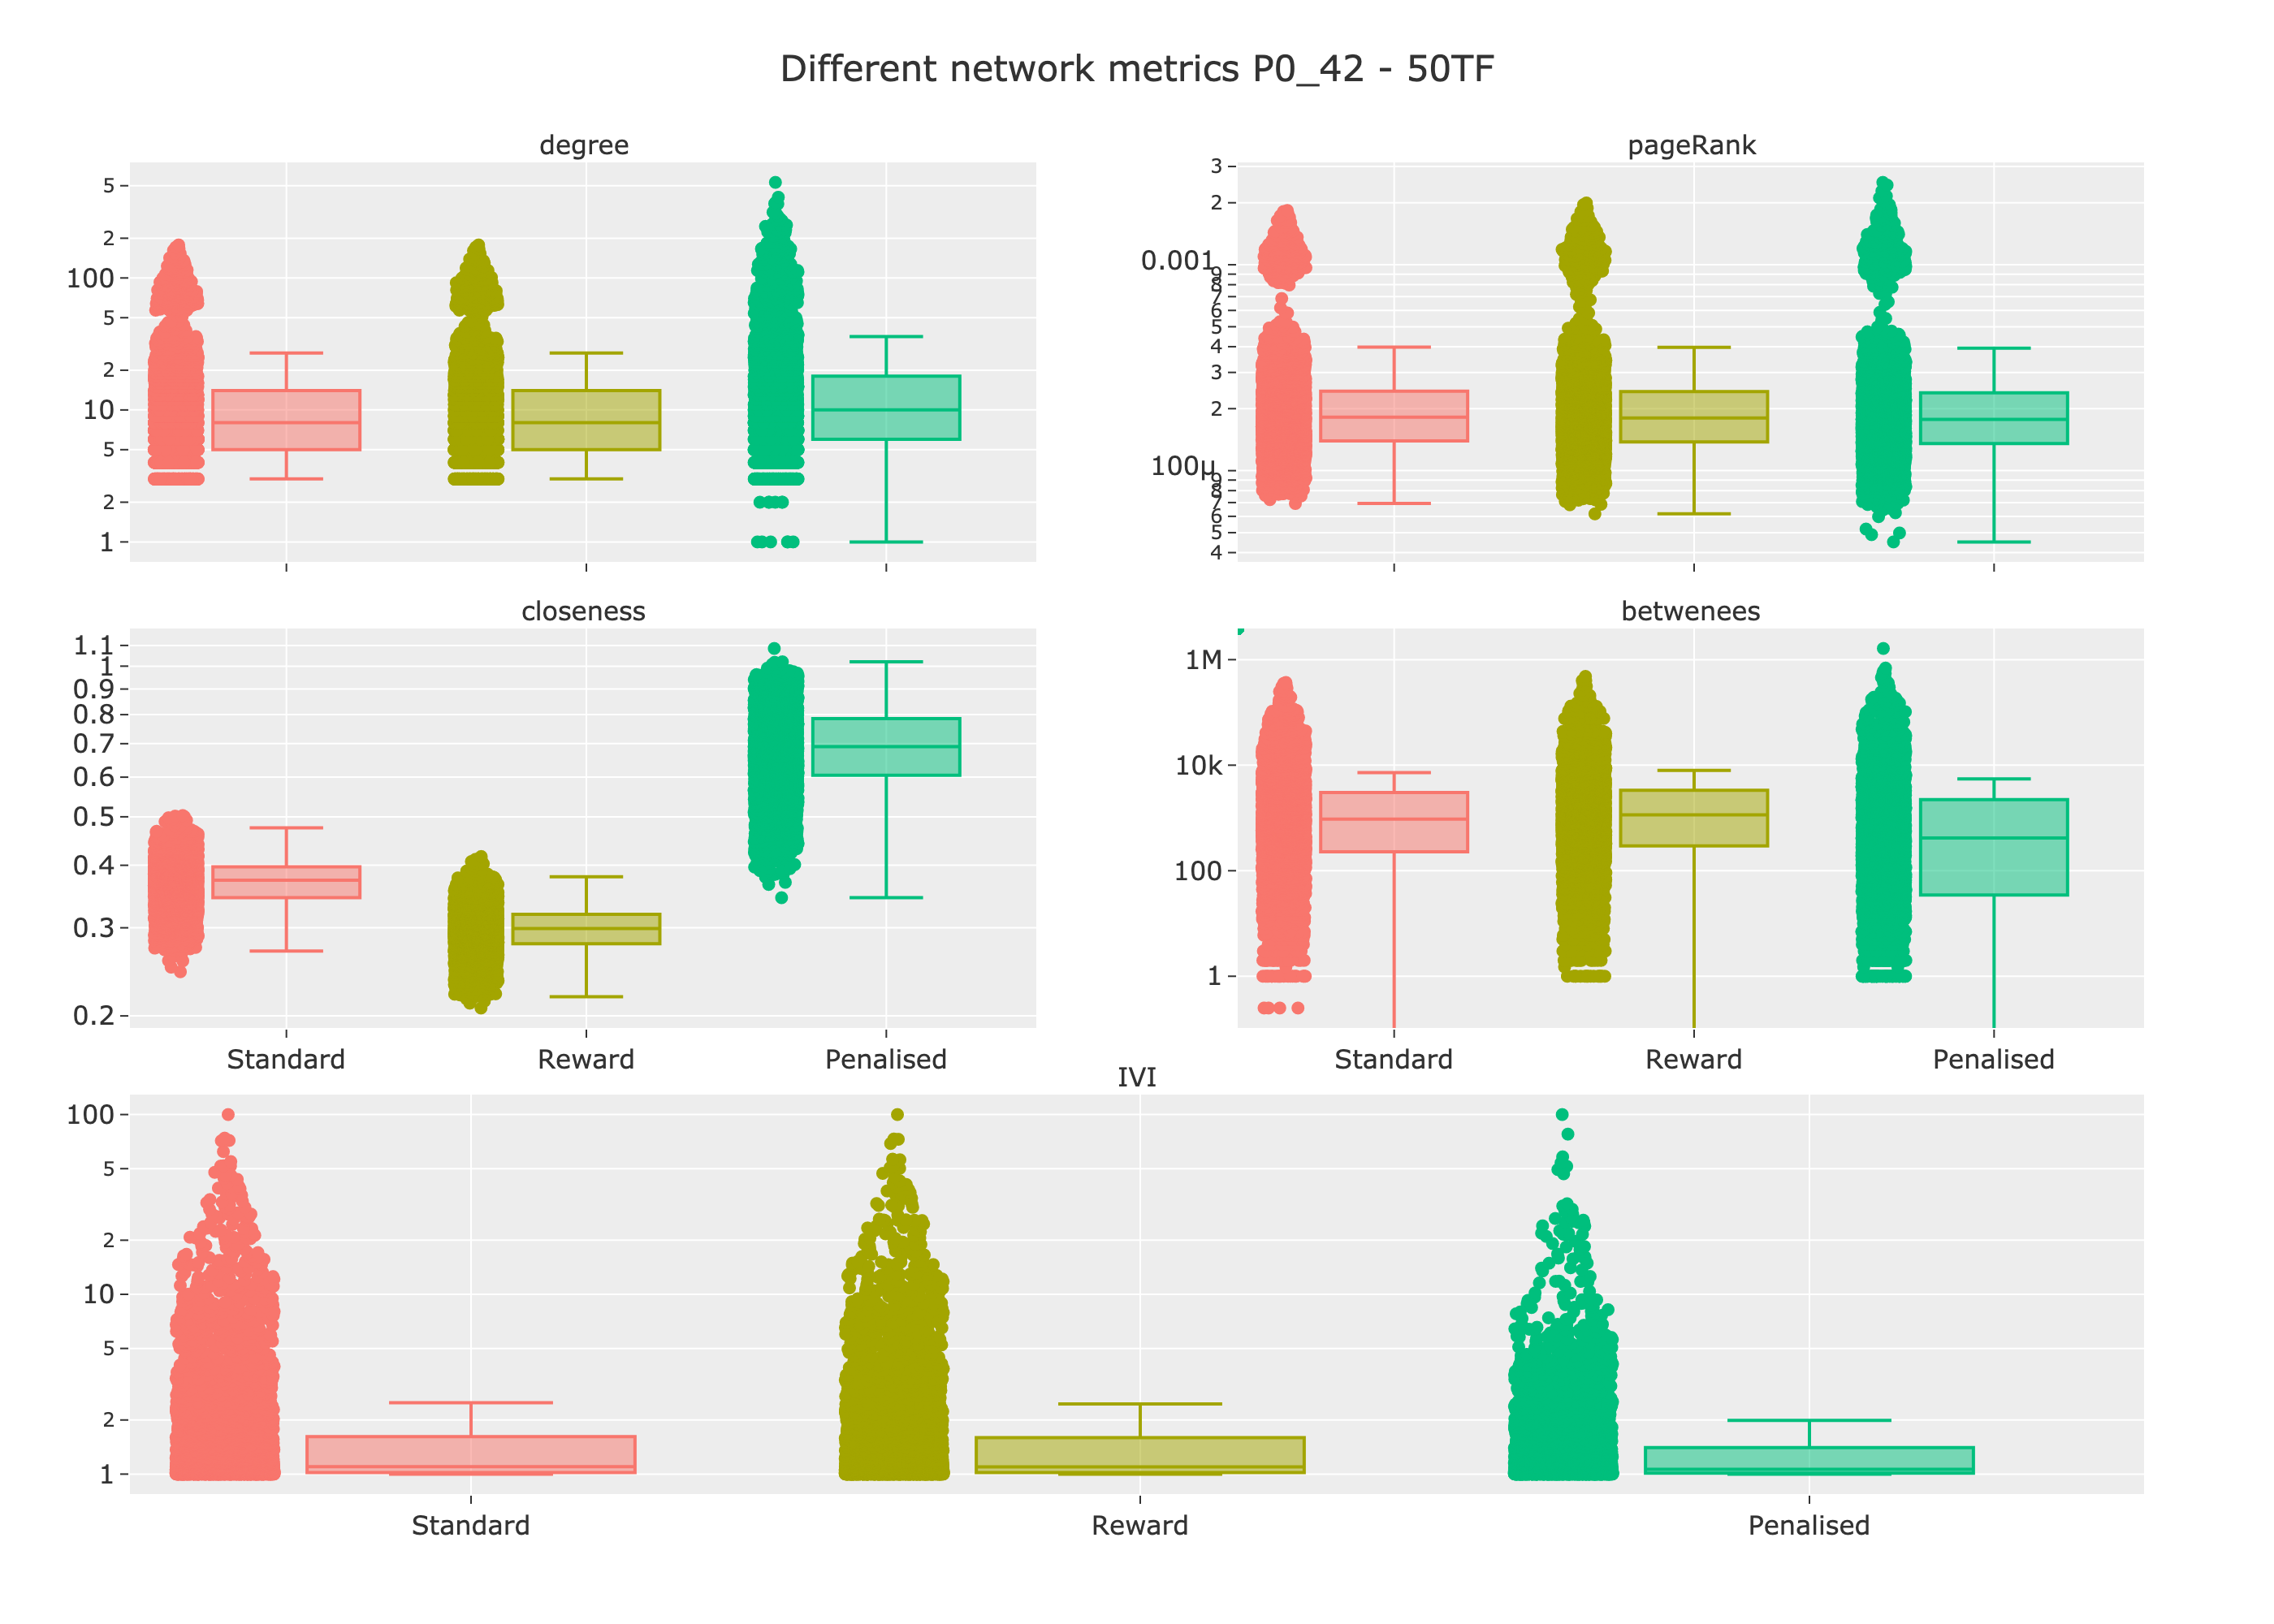
\includegraphics[width=1.0\textwidth,height=0.7\textheight,keepaspectratio]{Sections/Network_I/Resources/P0/P0_NetworkMetricsComp_50TF_2.png}
    \caption{Network metrics for the P0 networks formed from 4K genes, 3 connections per standard gene and 50 for TFs with the different weight modifiers; standard (red), reward (mustard) and penalised (green). The y-axis represent the log10 of the metric. }
    \label{fig:N_I:net_metrics_p0}
\end{figure}

In the previous section \ref{s:N_I:tum_describe}, five different network metrics were chosen to describe the networks generated: degree, PageRank, closeness, betweenness, and IVI. These metrics provide an overview of the network properties, how well the nodes are connected, the shortest path between them, and their overall importance (IVI). In Figure \ref{fig:N_I:net_metrics_p0}, the degree and PageRank plots for the Standard and Reward networks display a cone-shaped set of points, indicating a subgroup of genes with a high number of edges, while this is less evident in the Penalised network. It is also worth noting that the penalised modifier does not purge connections, which explains why the three networks have a similar mean degree. The graphs show similar means for the centrality, PageRank, and betweenness metrics, with the Penalised network exhibiting higher variance. This suggests that the Penalised networks may have more remote nodes. The Closeness figure shows that the Reward and Standard networks have lower values, which indicates the nodes are more spread out compared to the Penalised graph which vertices are closer. As for the Integrated Value of Influence (IVI), all networks have similar variance, mean, which indicates that the nodes local and global importance is not affected by the weight modifiers.

Overall, the network metrics indicate that the Penalised network is different from the other two networks, suggesting that reducing the weights to values close to 0 for highly mutated genes has a greater impact on the network than doubling their values. The largest impact on the network metric is on the closeness, the spread of the nodes' degree and betweenness. A similar behaviour was observed in the tumour networks in the previous section \cref{fig:N_I:net_metrics_tum}.

% Clustering model
\subsection{Choosing Clustering model} \label{s:p0:clustering_analysis}

% Explain what and why are the clustering methods we used
To find the appropriate clustering model and the number of clusters, the previous work from chapter \cref{s:cs:pre-processing}\footnote{Cluster analysis chapter} was adapted. This involved running Principal Component Analysis (PCA) and K-means to stratify MIBC based on gene expression. Based on three different clustering methods (Silhouette with cosine distance, Calinski-Harabasz, and Davies-Bouldin\footnote{For a refresher on the clustering metrics see \cref{s:lit:clustering_metrics})}, the following clustering models were selected\footnote{Other clustering methods explored included DBSCAN, MeanShift, Affinity Propagation, OPTICS, HDBSCAN, and Fuzzy K-means. The models kept are the ones which gave reasonable results; i.e. not clustering the samples only in 1 cluster or 2 clusters}. All models used the implementation on Scikit-learn \cite{Scikit-learn_undated-ax}: K-means, Agglomerative Clustering with Average linkage (Agg\_Avg), Ward, Gaussian Mixture Model, and Spectral Clustering.

\begin{figure}[!htb]
    \centering
    \begin{subfigure}[!t]{0.49\textwidth}
        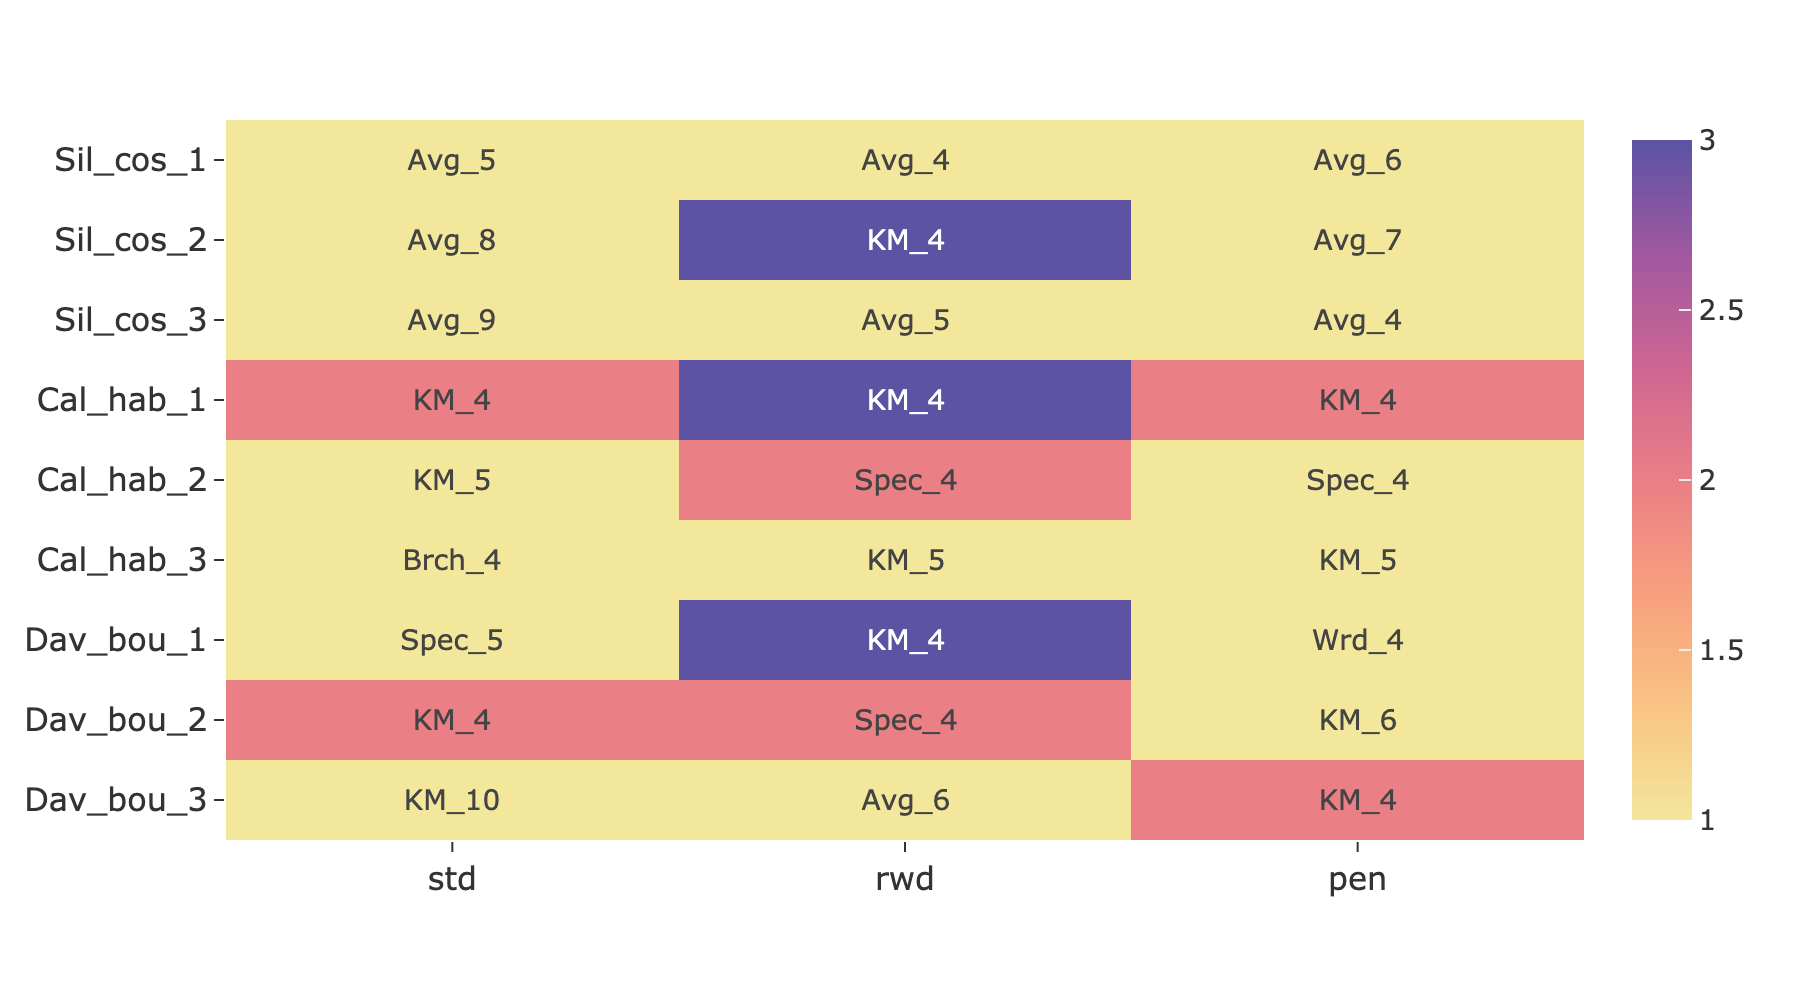
\includegraphics[width=\textwidth,keepaspectratio]{Sections/Network_I/Resources/P0/top3_cs_gen_p0_tum4K_50TF_v3.png}    
        \caption{Cluster model and size}
        \label{fig:N_I:p0_metr_model_size}
    \end{subfigure}
    \begin{subfigure}[!t]{0.49\textwidth}
        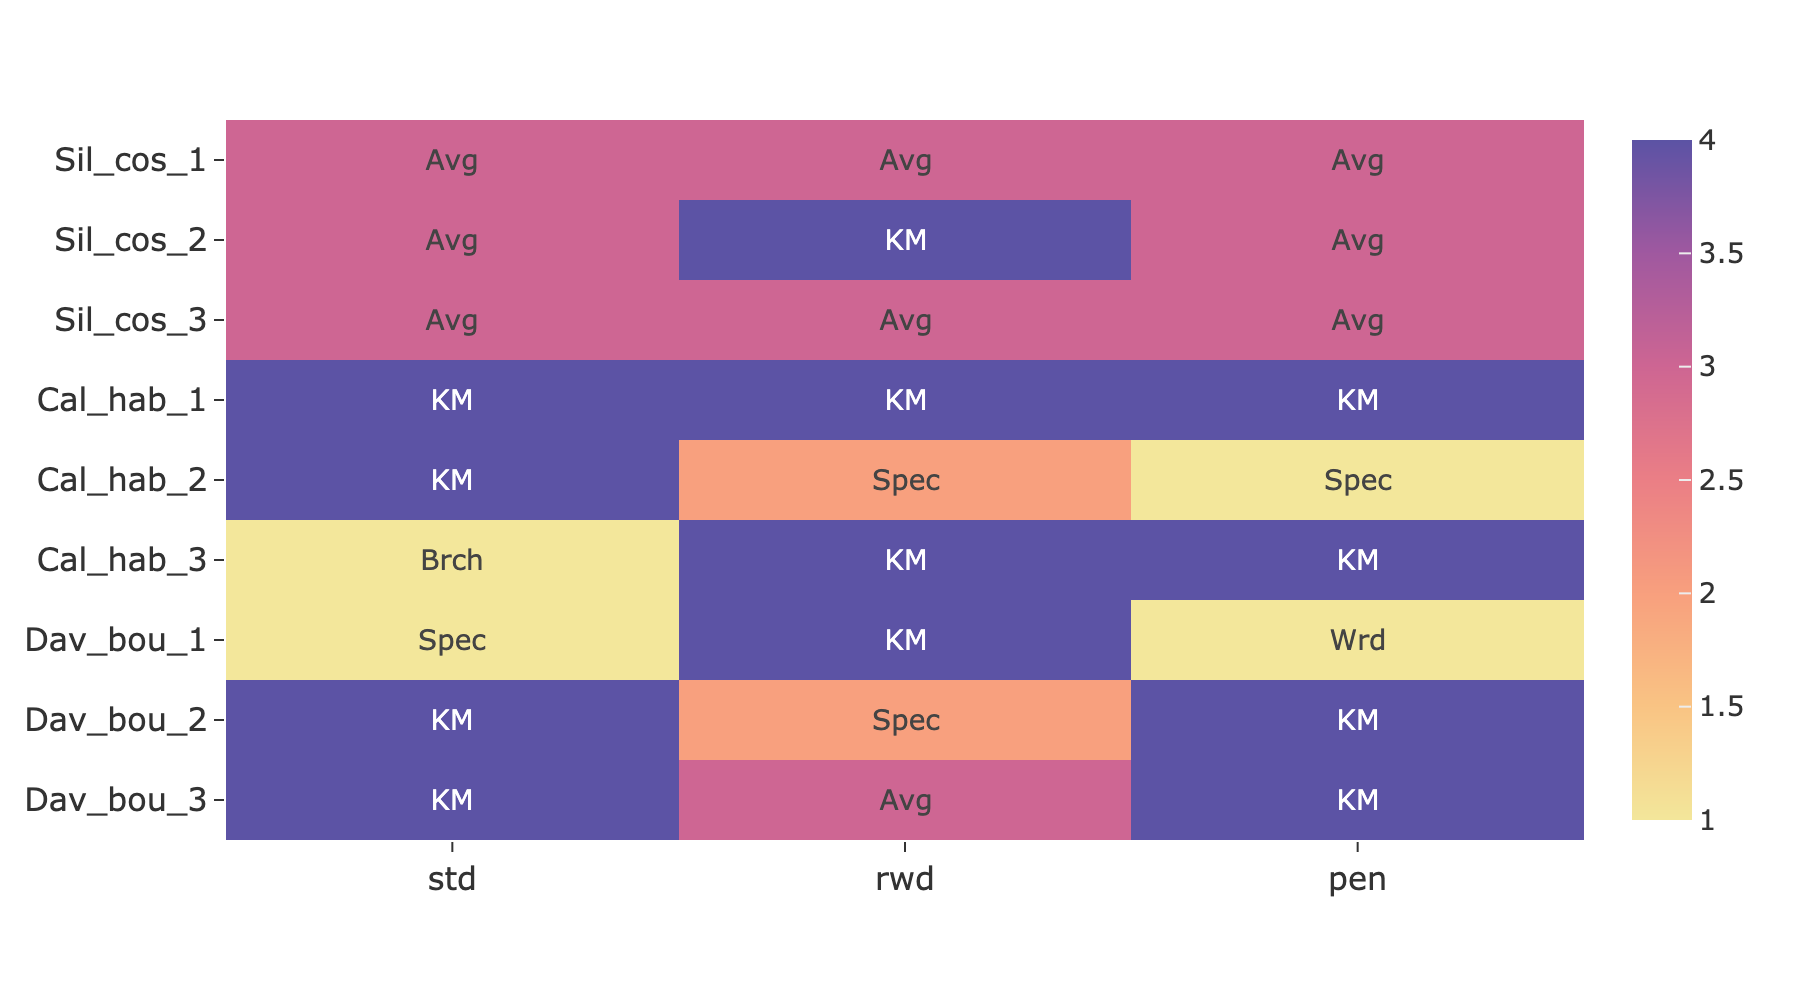
\includegraphics[width=\textwidth,keepaspectratio]{Sections/Network_I/Resources/P0/top3_cs_model_p0_tum4K_50TF_v3.png}
        \caption{Cluster model}
        \label{fig:N_I:p0_metr_model}
    \end{subfigure} 
    \begin{subfigure}[!t]{0.49\textwidth}
        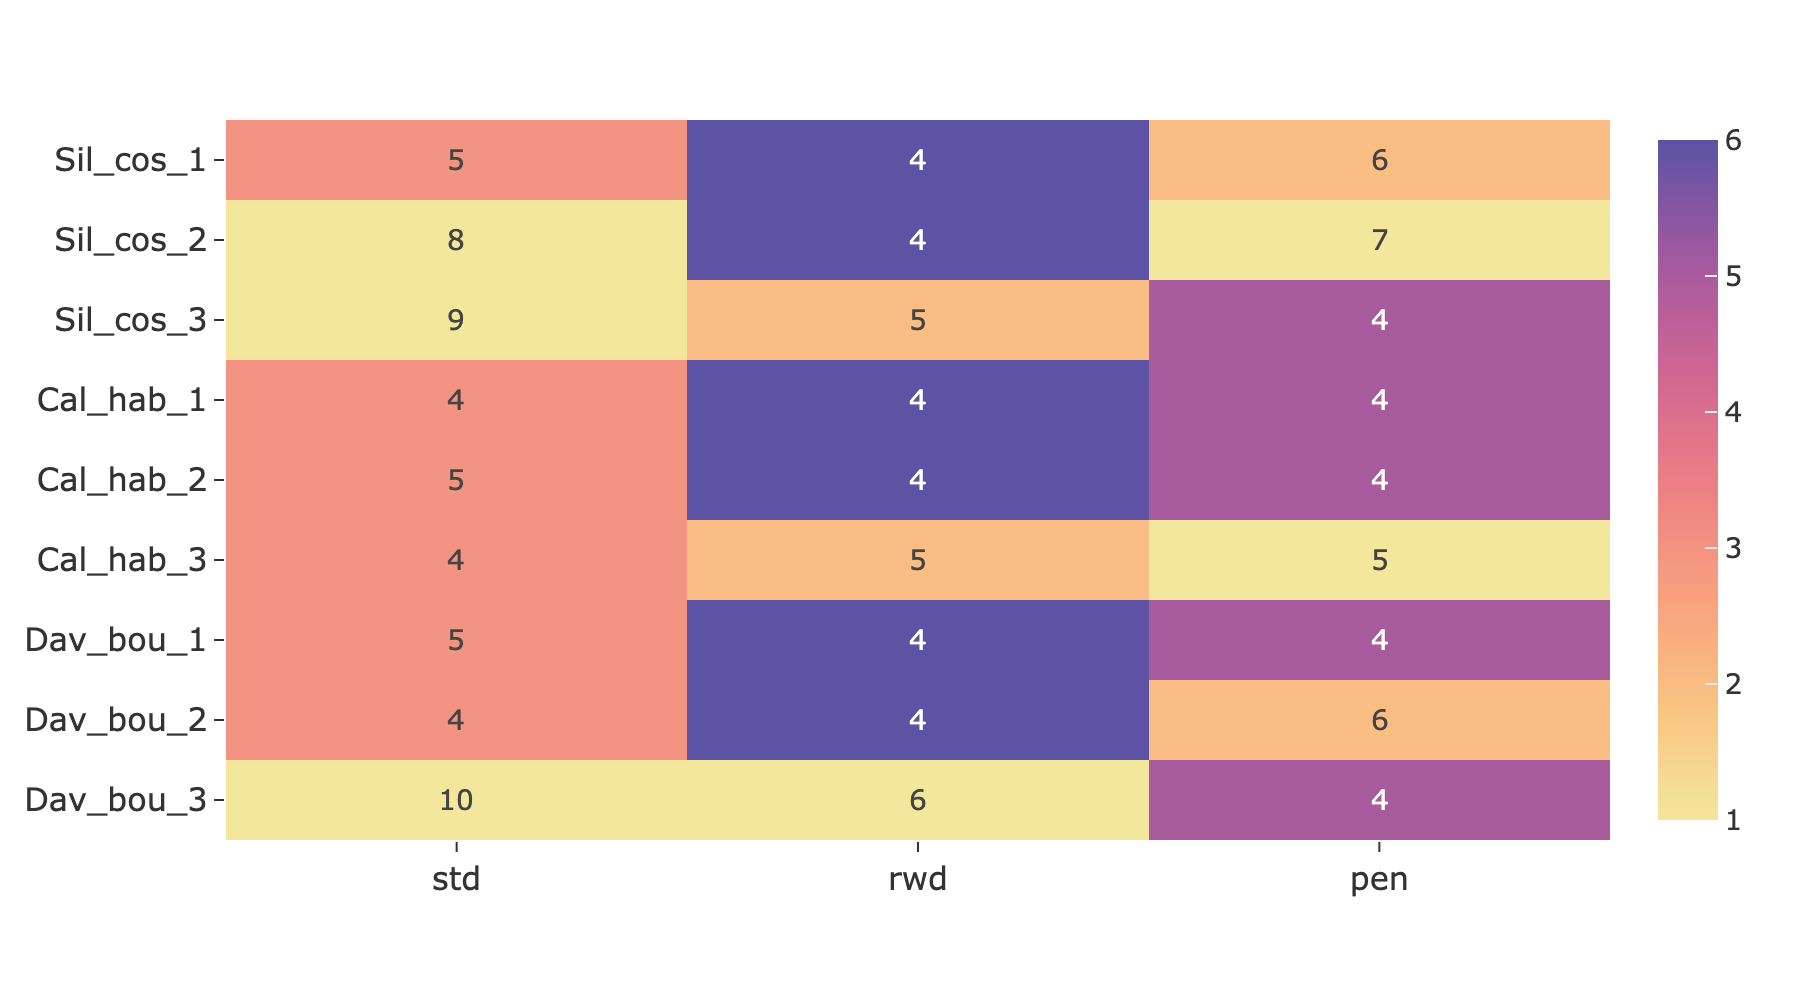
\includegraphics[width=\textwidth,keepaspectratio]{Sections/Network_I/Resources/P0/top3_cs_size_p0_tum4K_50TF_v3.png}
        \caption{Cluster size}
        \label{fig:N_I:p0_metr_size}
    \end{subfigure}
    \begin{subfigure}[!t]{0.49\textwidth}
        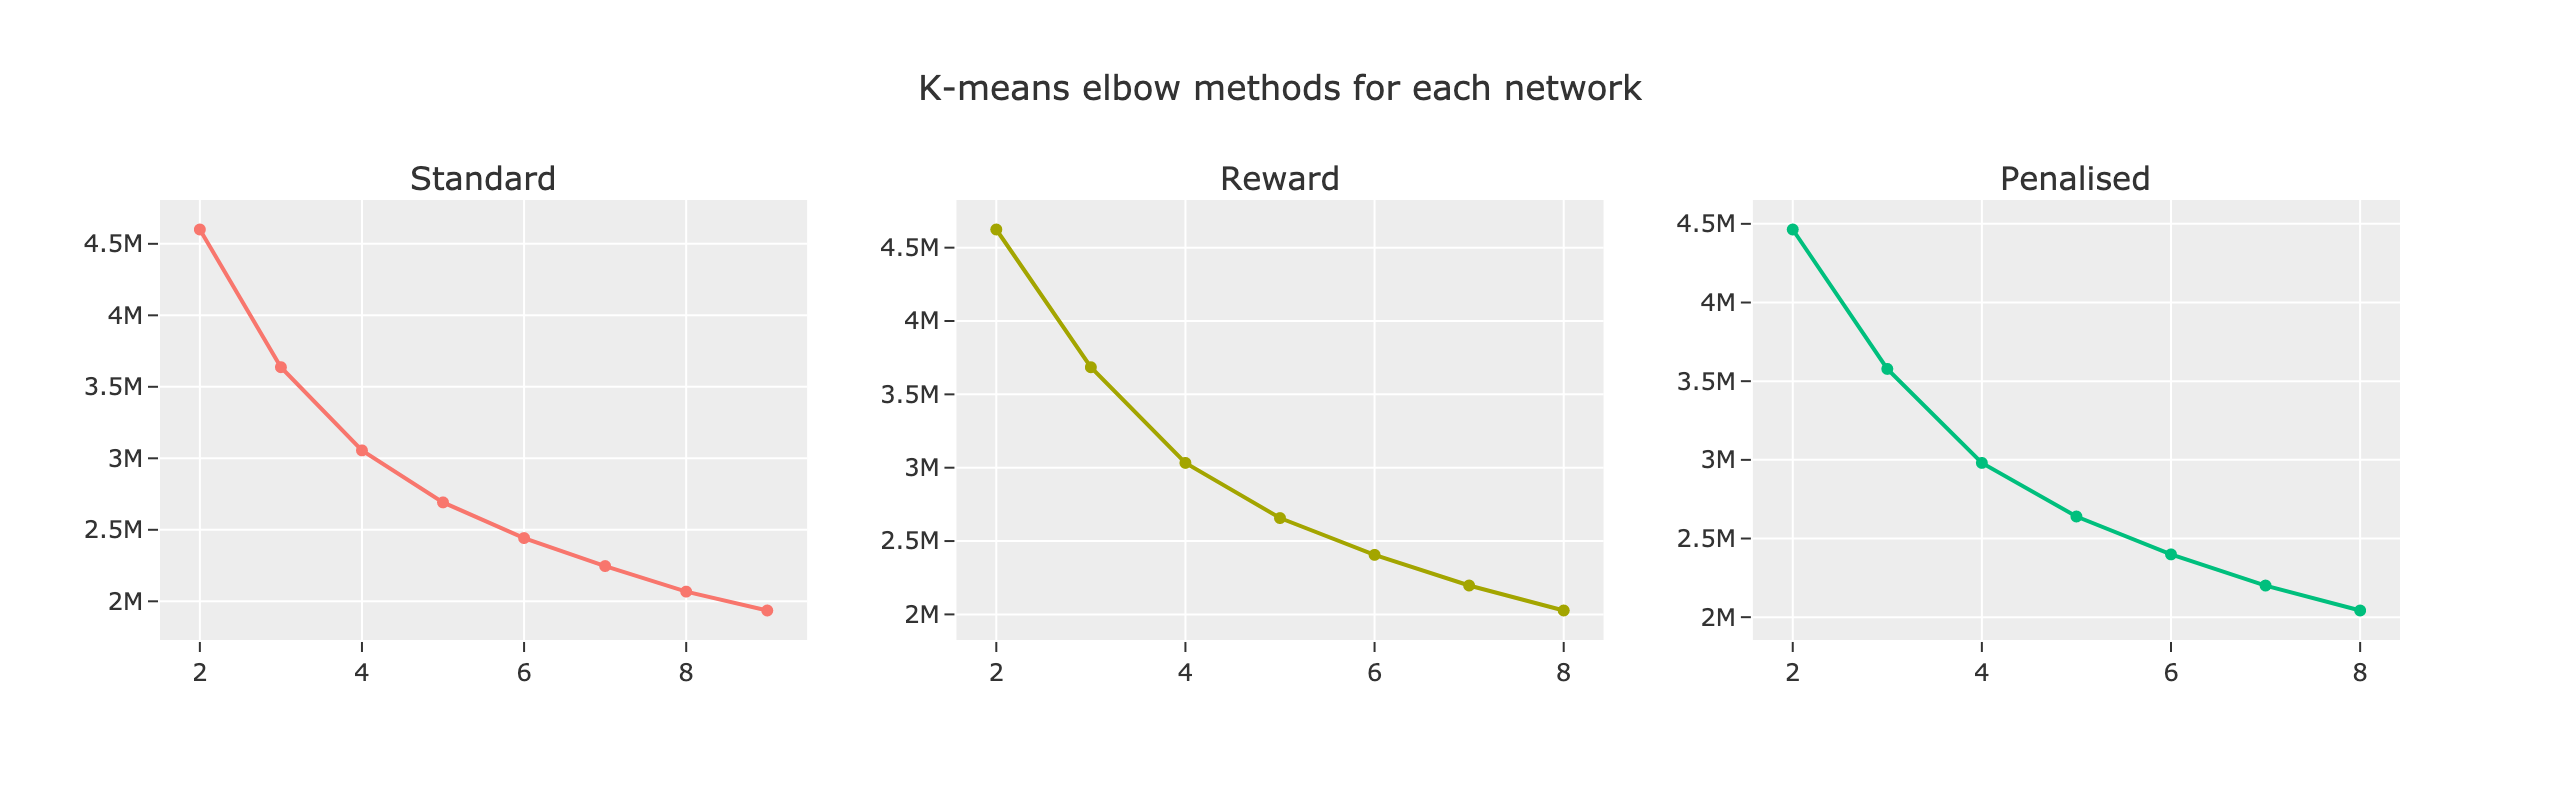
\includegraphics[width=\textwidth, keepaspectratio]{Sections/Network_I/Resources/P0/p0_elbowMethod_4K_v3.png}
        \label{fig:N_I:p0_elbow_method}
        \caption{Elbow method}
    \end{subfigure}
    \caption{Clustering models for each network type with the top three clustering scores. Colouring scale corresponds to the encounter frequency \textbf{per network type}; i.e. the count restarts for every network. A) looks at the overall most common clustering model configuration. B) at the most common clustering model C) the most likely cluster size.}
    \label{fig:N_I:p0_top_3_metrics}
\end{figure}

% Introduce the results and motivate the reason why we don't include K=2,3
The clustering methods were applied to the MEV scores derived from the three networks (Standard, Reward, and Penalised) with K ranging from 3-9, and the same clustering metrics were used to assess performance. Models with 2 or 3 clusters were not considered, as the metrics tend to give higher scores for models with 2 or 3 clusters. In \cref{fig:ap:p0_choosing_cs} in the Appendix, the clustering metrics for the chosen models are displayed, with the number of 'x' marking the highest score after cluster sizes 2 and 3. The plot shows that there is a proportional decrease in performance by the metrics with the increase in K. 

While \cref{fig:ap:p0_choosing_cs} shows the general trends of the metrics across the 3 different clustering scores, it is not very clear which model with how many clusters performs the best for each network or overall.

\begin{figure}[!htb]

    \centering
    \begin{subfigure}{1.0\linewidth}
        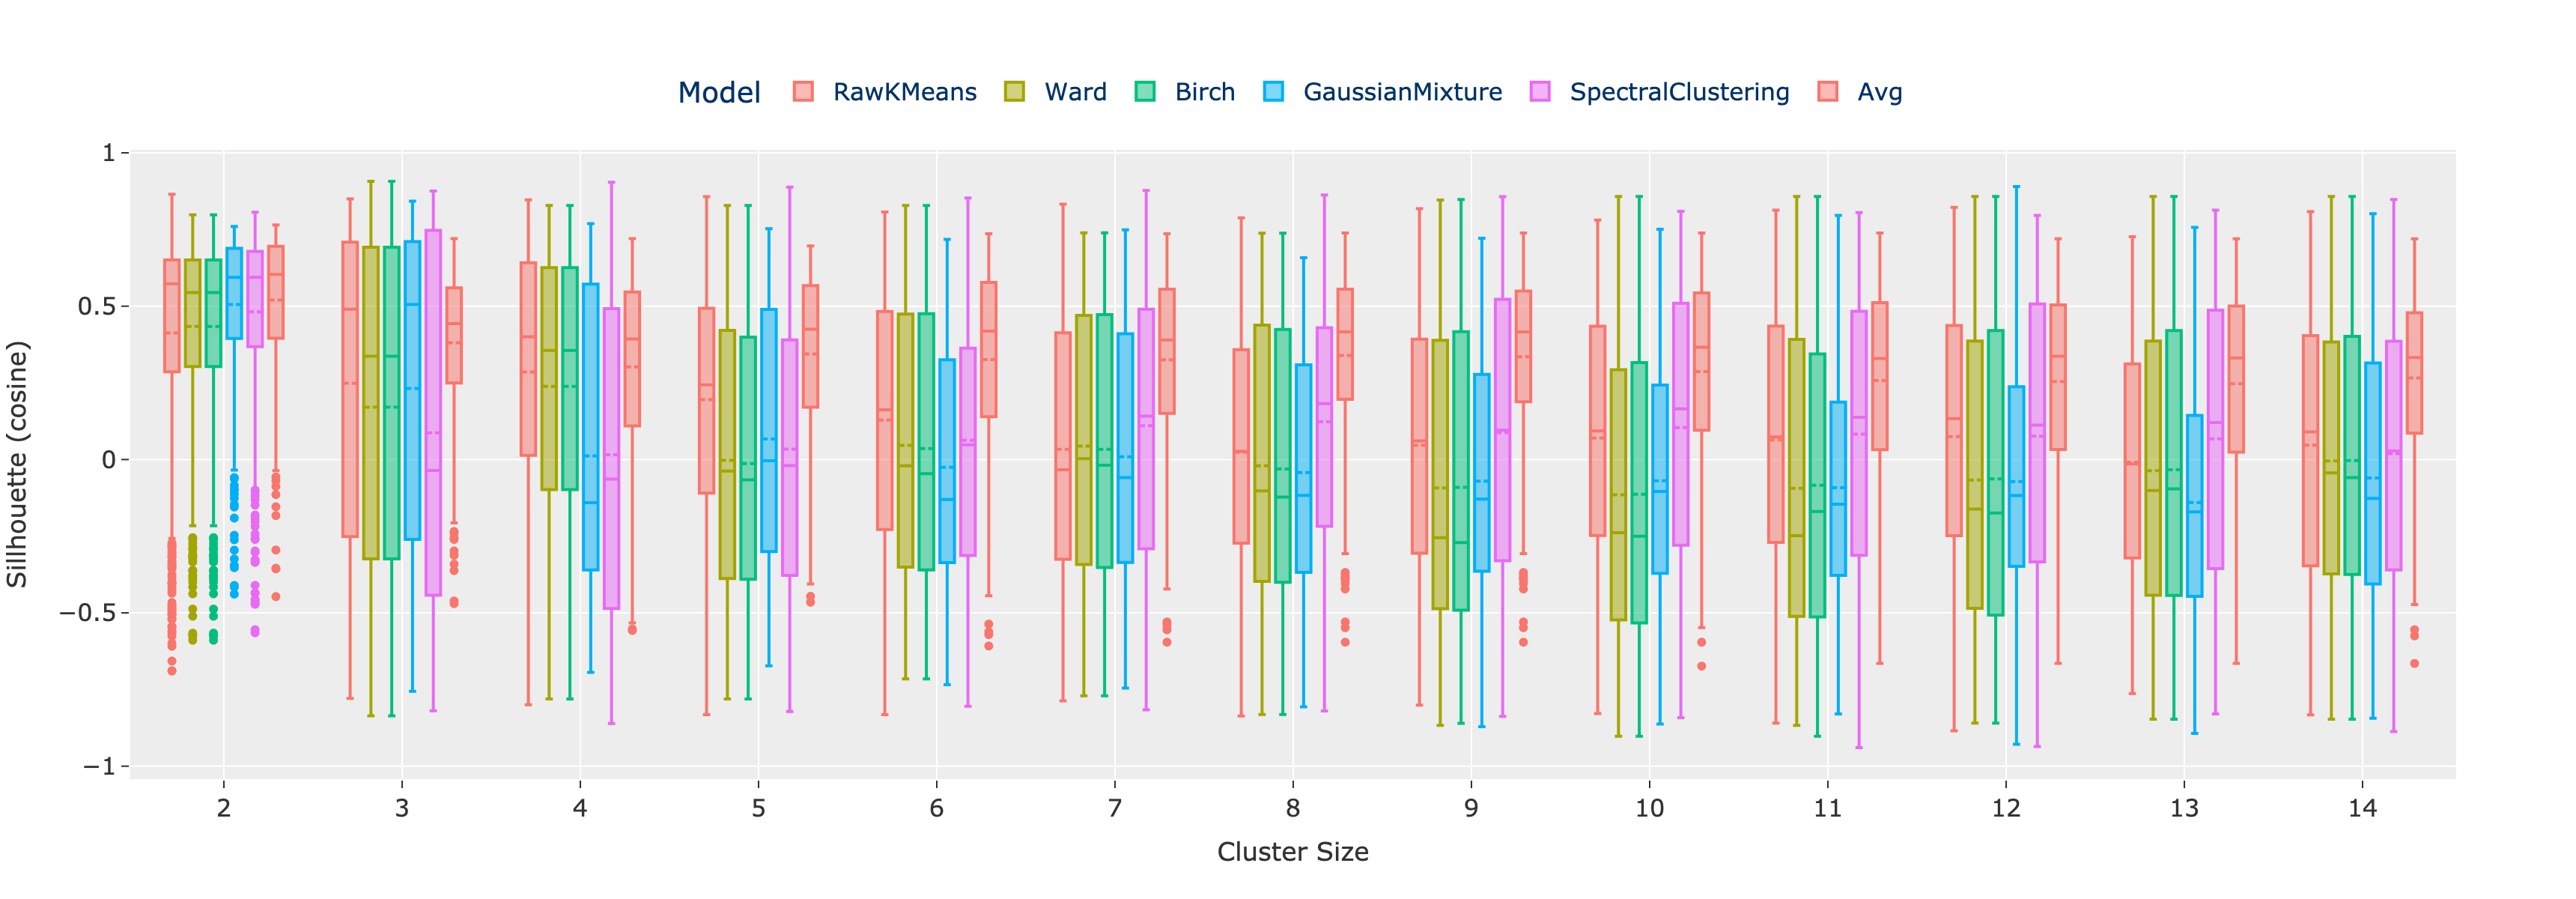
\includegraphics[width=1.0\textwidth,keepaspectratio]{Sections/Network_I/Resources/P0/std_tum4k_v3_sill_spread.png}
        \caption{Standard network}
        \label{fig:N_I:p0_sill_std}
    \end{subfigure} %
    \centering
    \begin{subfigure}{1.0\linewidth}
        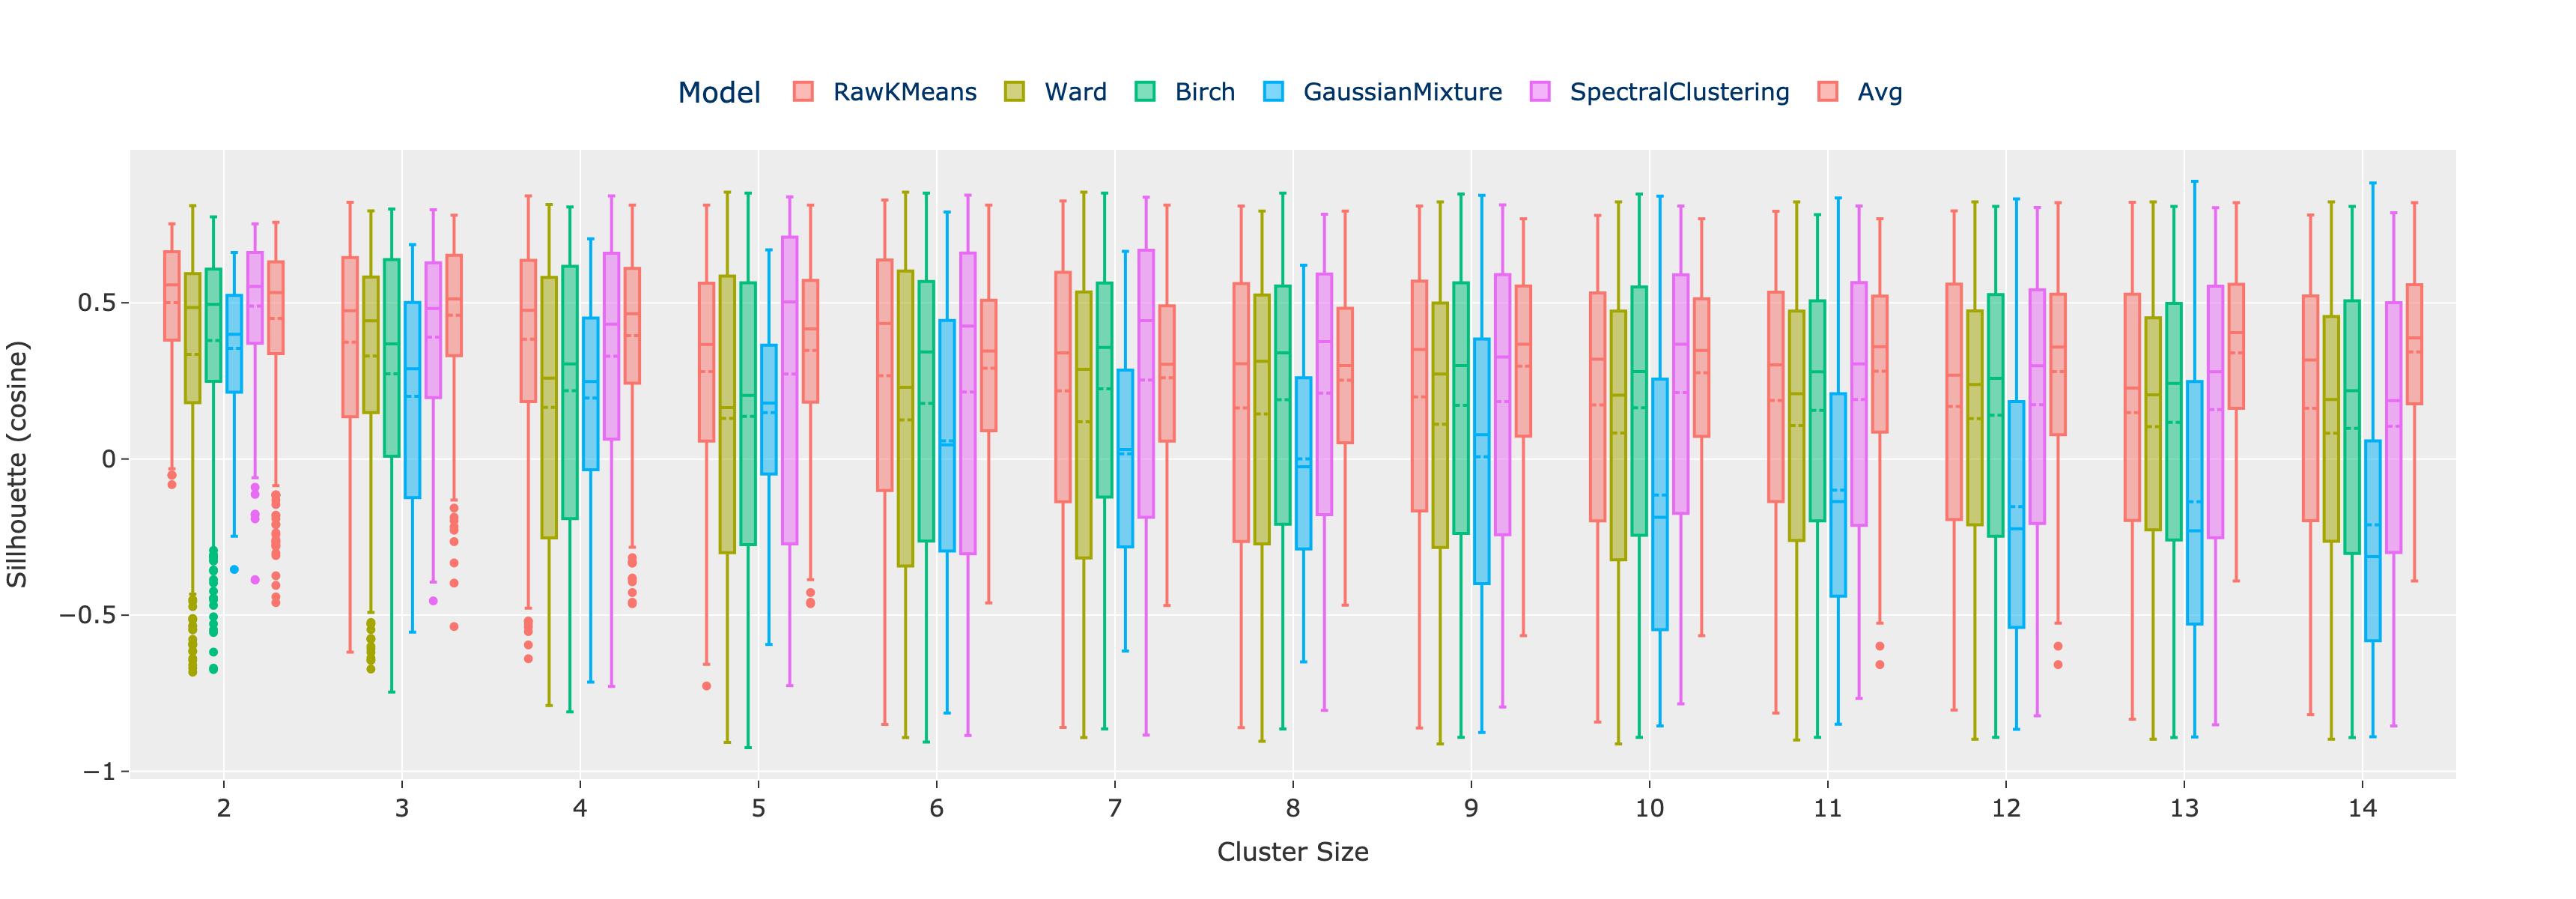
\includegraphics[width=1.0\textwidth,keepaspectratio]{Sections/Network_I/Resources/P0/rwd_tum4k_v3_sill_spread.png}
        \caption{Reward network}
        \label{fig:N_I:p0_sill_rwd}
    \end{subfigure}
    \centering
    \begin{subfigure}{1.0\linewidth}
        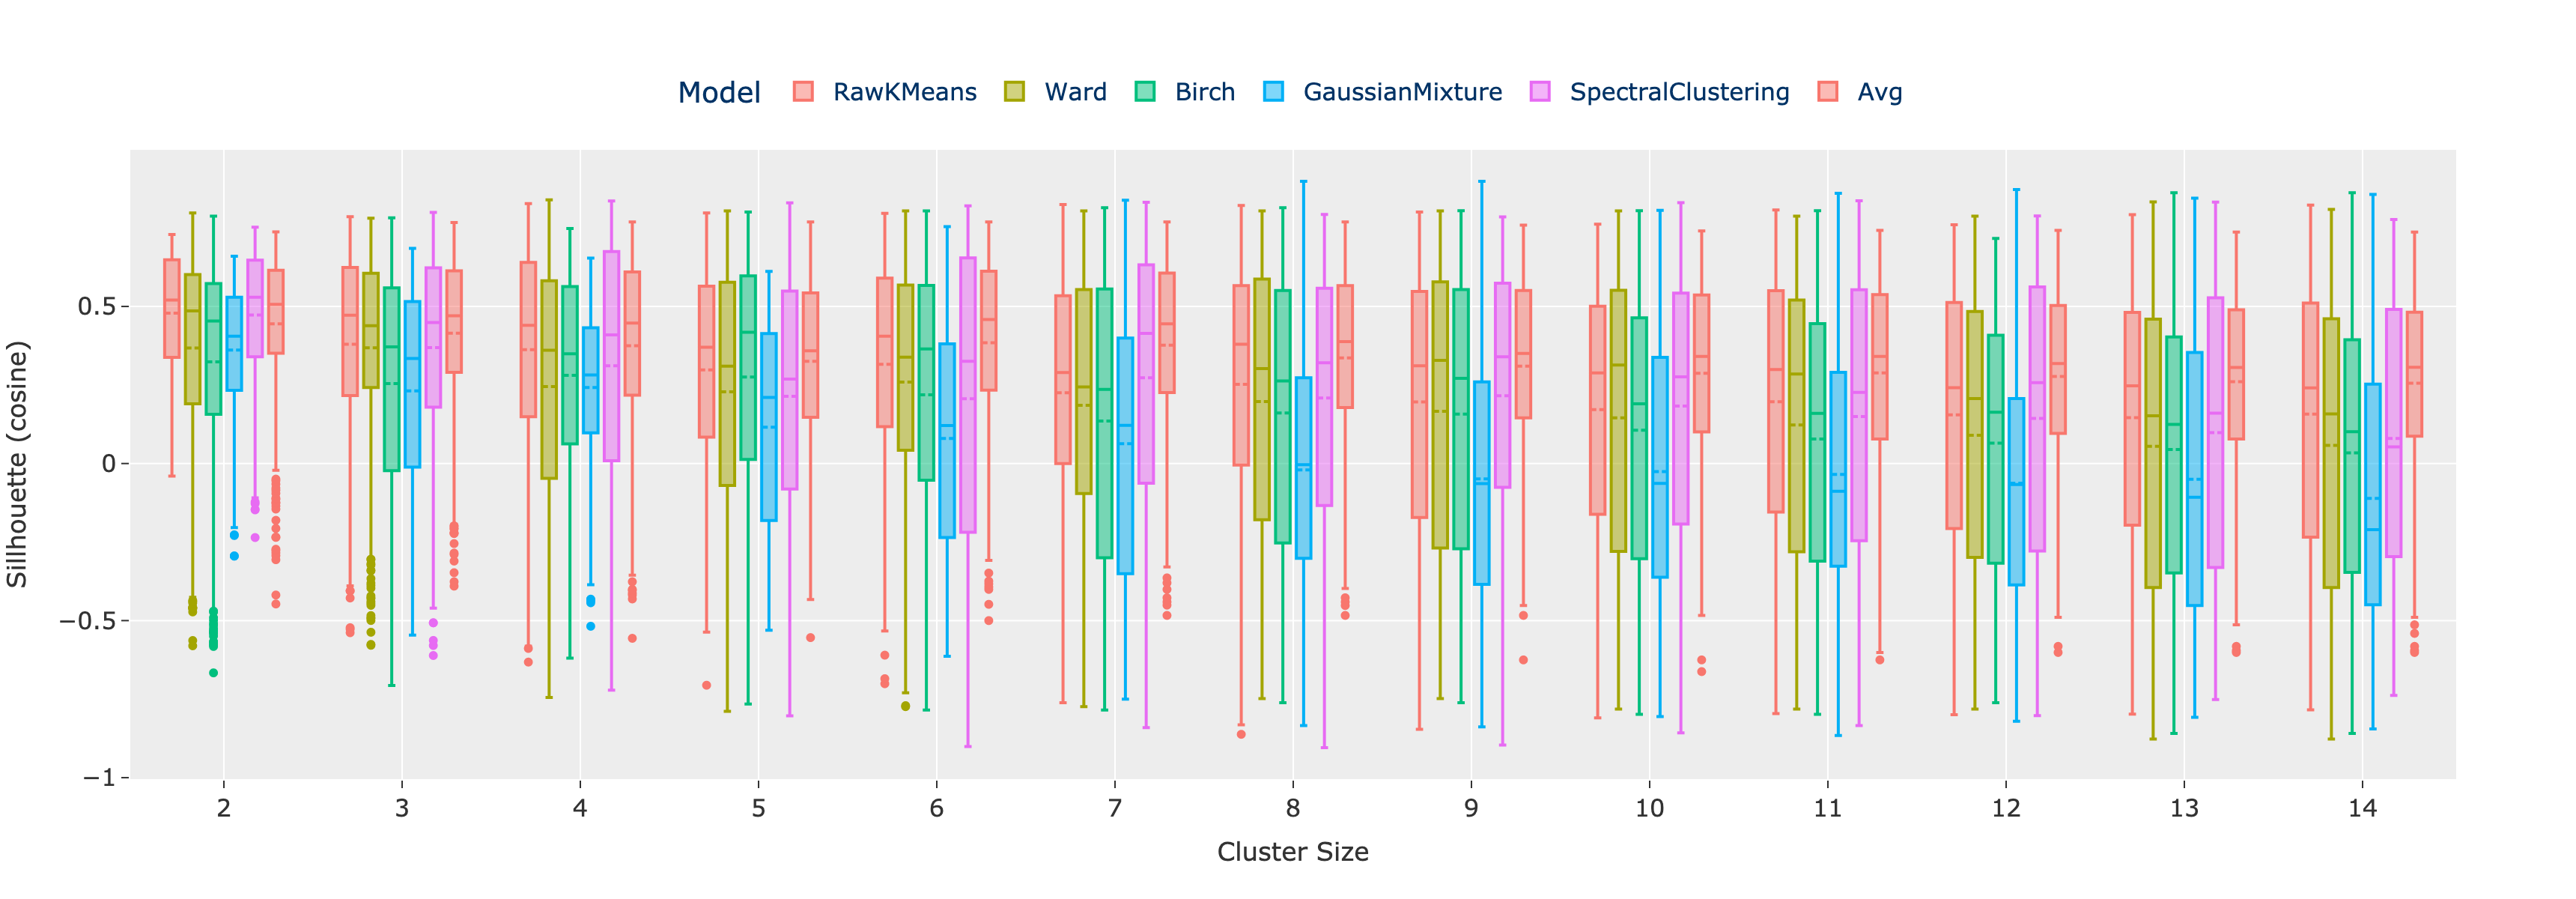
\includegraphics[width=1.0\textwidth,keepaspectratio]{Sections/Network_I/Resources/P0/pen_tum4k_v3_sill_spread.png}      
        \caption{Penalised network}
        \label{fig:N_I:p0_sill_pen}
    \end{subfigure}
    \caption{Cosine Silhouette score spread across samples over different clustering models with various K.}
    \label{fig:N_I:p0_sillhouette_spread}
\end{figure}

% Comment on Top 3 models + cs, models and just CS
\Cref{fig:N_I:p0_top_3_metrics} assists decision making by depicting both the most used cluster model and number of clusters in \cref{fig:N_I:p0_metr_model_size}, and separately the cluster model and size in \cref{fig:N_I:p0_metr_model,fig:N_I:p0_metr_size}; the colouring scale corresponds to the encounter frequency across network type (i.e. per column). For example, in \cref{fig:N_I:p0_metr_model_size} K-means with K=4 appears three times across the reward graph, and Spectral Clustering with K=4 appears two times in all three network types. The colouring strategies help delineate the configurations for each network.

From \cref{fig:N_I:p0_metr_model_size}, which shows the combined model and K, it can be observed that the reward network is the only one having a model picked by all three metrics. In \cref{fig:N_I:p0_metr_model}, Agg\_Avg scores very high in the cosine metric, while K-means generally performs better according to the other metrics. \Cref{fig:N_I:p0_metr_size}, K=4 is the preferred number of clusters for the reward and penalised networks, while the standard network oscillates between 4 and 5. Overall, the clustering scores suggest that both K-means and Agg\_Avg have similar performances, with the preferred cluster size being K=4, followed by K=5. Furthermore, K=4 is the overall choice of cluster numbers through the heuristic approach of the elbow method in \cref{fig:N_I:p0_elbow_method} 


% Using cosine sillhouette to look at the spread
The lack of an obvious cluster model shows the challenge of working with gene expression datasets. It also shows the limitation of using average scores for clustering metrics. Thus, the Silhouette cosine score is selected\footnote{For the same reason as we chosen it as a main metric in the last chapter. Compared with the other metrics the Silhouette score uses cosine as a distance which is more suitable for high dimension data.} to explore the variance across samples in Figure \cref{fig:N_I:p0_sillhouette_spread}. With the exception of the Agg\_Avg and K-means the other clustering models have a higher spread of the silhouette across the different cluster size.

% narrowing done to the 2 clustering models
The clustering scores and the analysis performed suggests that K-means and Agglomerative Clustering with average linkage perform better than the rest as in the top 3 models used in \cref{fig:N_I:p0_metr_model} and the silhouette spread in Figure \cref{fig:N_I:p0_sillhouette_spread}. The Elbow method form \cref{fig:N_I:p0_elbow_method} and the other metrics suggests that K=4 is the right choice. This is different from what is expected as in the earlier work \cref{s:clustering_analysis} at least five clusters were found, using computational methods and K=6 with biological knowledge (IFNg groups). On top of that, this is is the next K considered as K=2,3 were not considered as these will always exhibit the best K.

\begin{figure}[!htb]
    \centering
    \begin{subfigure}[b]{0.8\textwidth}
        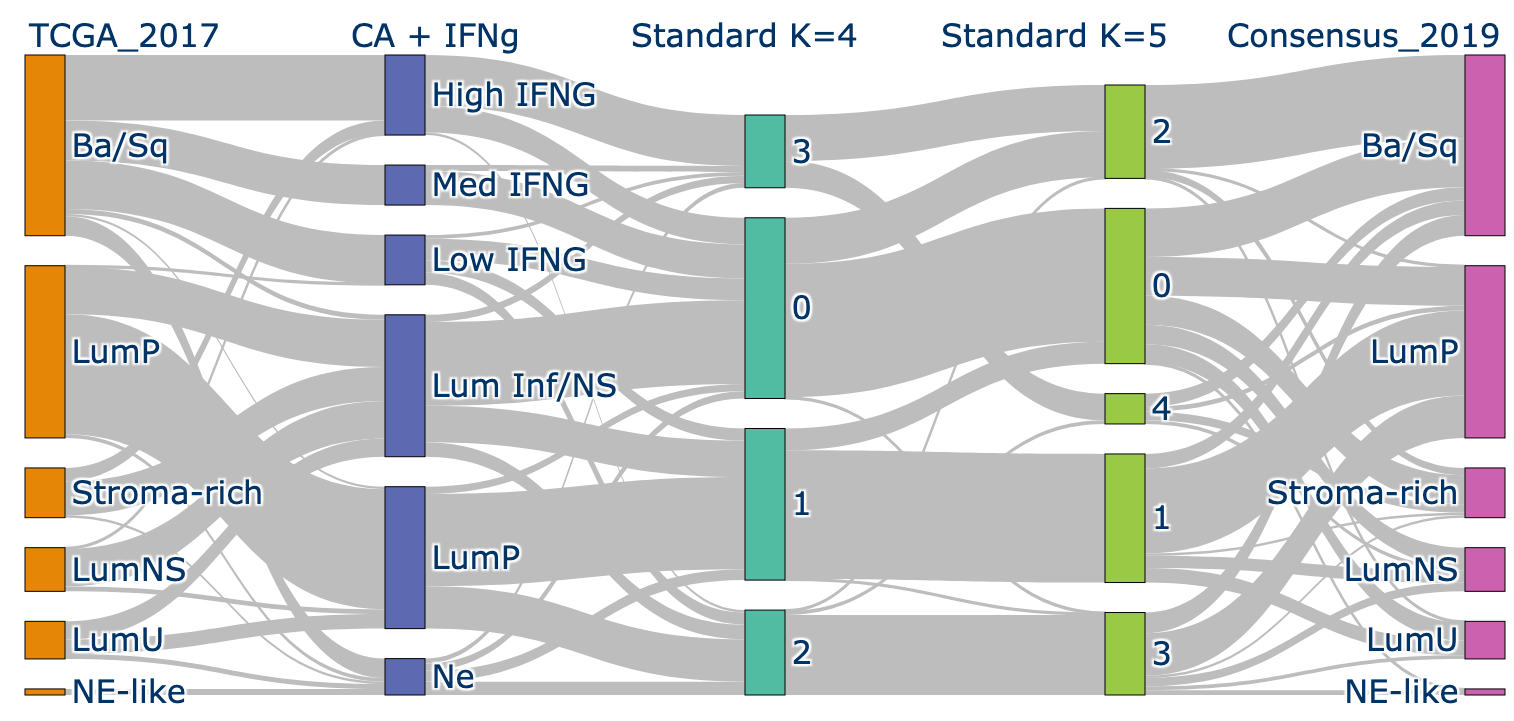
\includegraphics[width=\textwidth,keepaspectratio]{Sections/Network_I/Resources/P0/Sankey_KM_4K_v3.png}
        \label{fig:N_I:p0_sky_KM}
        \caption{K-Means}
    \end{subfigure}
    \begin{subfigure}[b]{0.8\textwidth}
        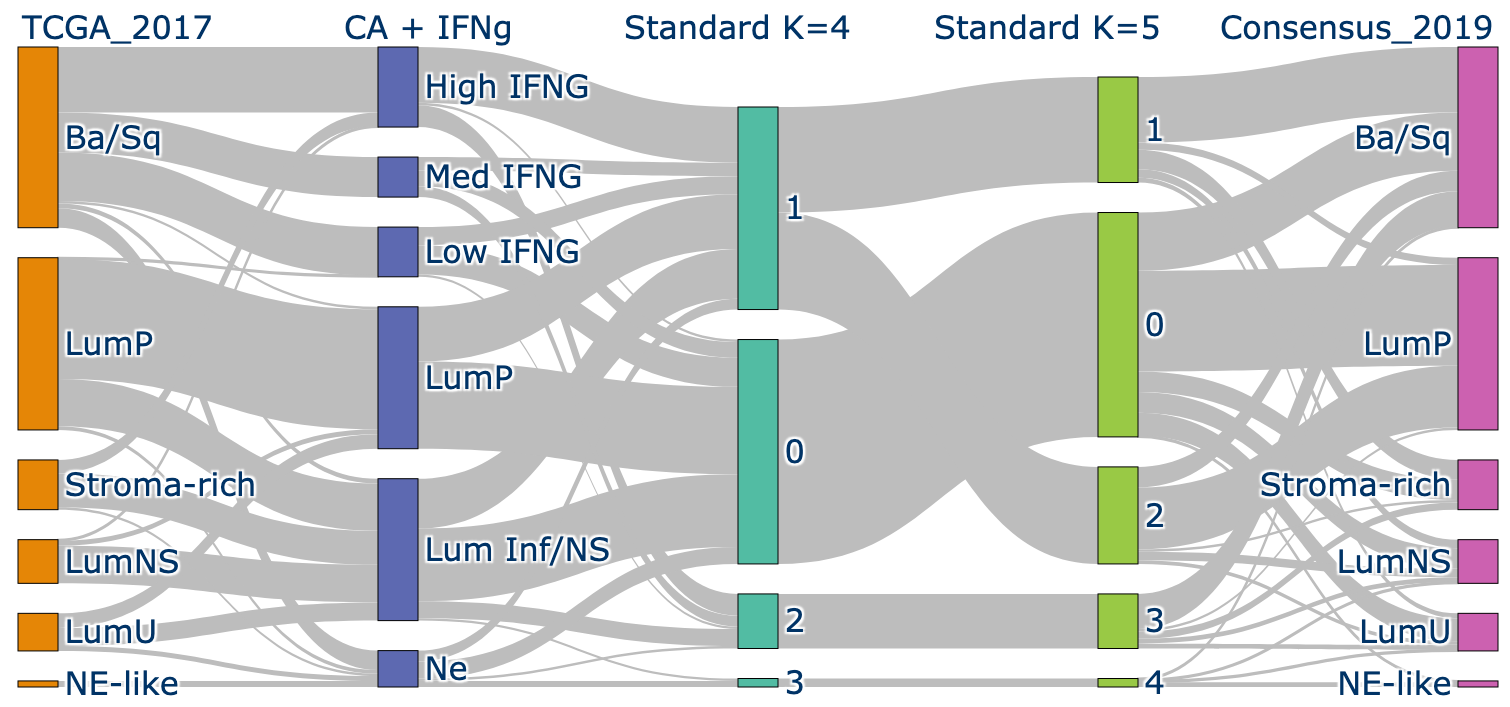
\includegraphics[width=\textwidth,keepaspectratio]{Sections/Network_I/Resources/P0/Sankey_Avg_4K_v3.png}
        \caption{Agglomerative with average linkage}
        \label{fig:N_I:p0_sky_AGG}
    \end{subfigure}
    \caption{Sankey plots for the two best performing models. }
    \label{fig:N_I:p0_sky_Agg_KMeans}
\end{figure}


Two Sankey plots in \cref{fig:N_I:p0_sky_Agg_KMeans} are used to assess the differences in the MIBC subtyping between the two best clustering model and the two cluster sizes\footnote{The standard networks were the ones only used for comparison to simplify the process.}. There is a striking difference between the two clustering models, Agg\_Avg finds disproportionate clusters while the K-means finds similar size groups. This, together with the High IFNG subgroup found by K-means suggests that this clustering model is the appropriate choice. 

The cluster metrics are not informative in determining the number of clusters, the scores decrease proportionally with the number of clusters, resulting in the lowest K giving the best result. Elbow method complements the metrics but it is a heuristic approach. When K=5, for the K-means, the Basal groups seems to be better defined by having a smaller group (4) and a large one (2). For this, and the fact that previous work in the PhD showed that there there should be more groups, K-means with K=5 is preferred over K=4.

% Network comparison
\subsection{Network comparison}


\Cref{fig:N_I:p0_sky_leiden} represents an overview of the decisions made in the previous sub-section, K-means (K=5) was found to be the most suitable clustering model. The three networks are compared with the consensus and TCGA classifiers \citet{Kamoun2020-tj, Robertson2017-mg} as well as our subtyping from the cluster analysis section \cref{s:clustering_analysis}. From the top left figure it can be observed that the number of communities is similar across the three networks, there are 9 or 10 blocks, with a few exceptions. There are significantly less communities compared with the number of subgraphs found in the tumour network; see Figure \ref{fig:N_I:tum_leiden_modifiers}. The small variance of the Modularity score in the Figure on the right suggests that the communities are fairly stable and the penalised network have a lower performance by 0.04.

\begin{figure}[!t]    
    \centering
    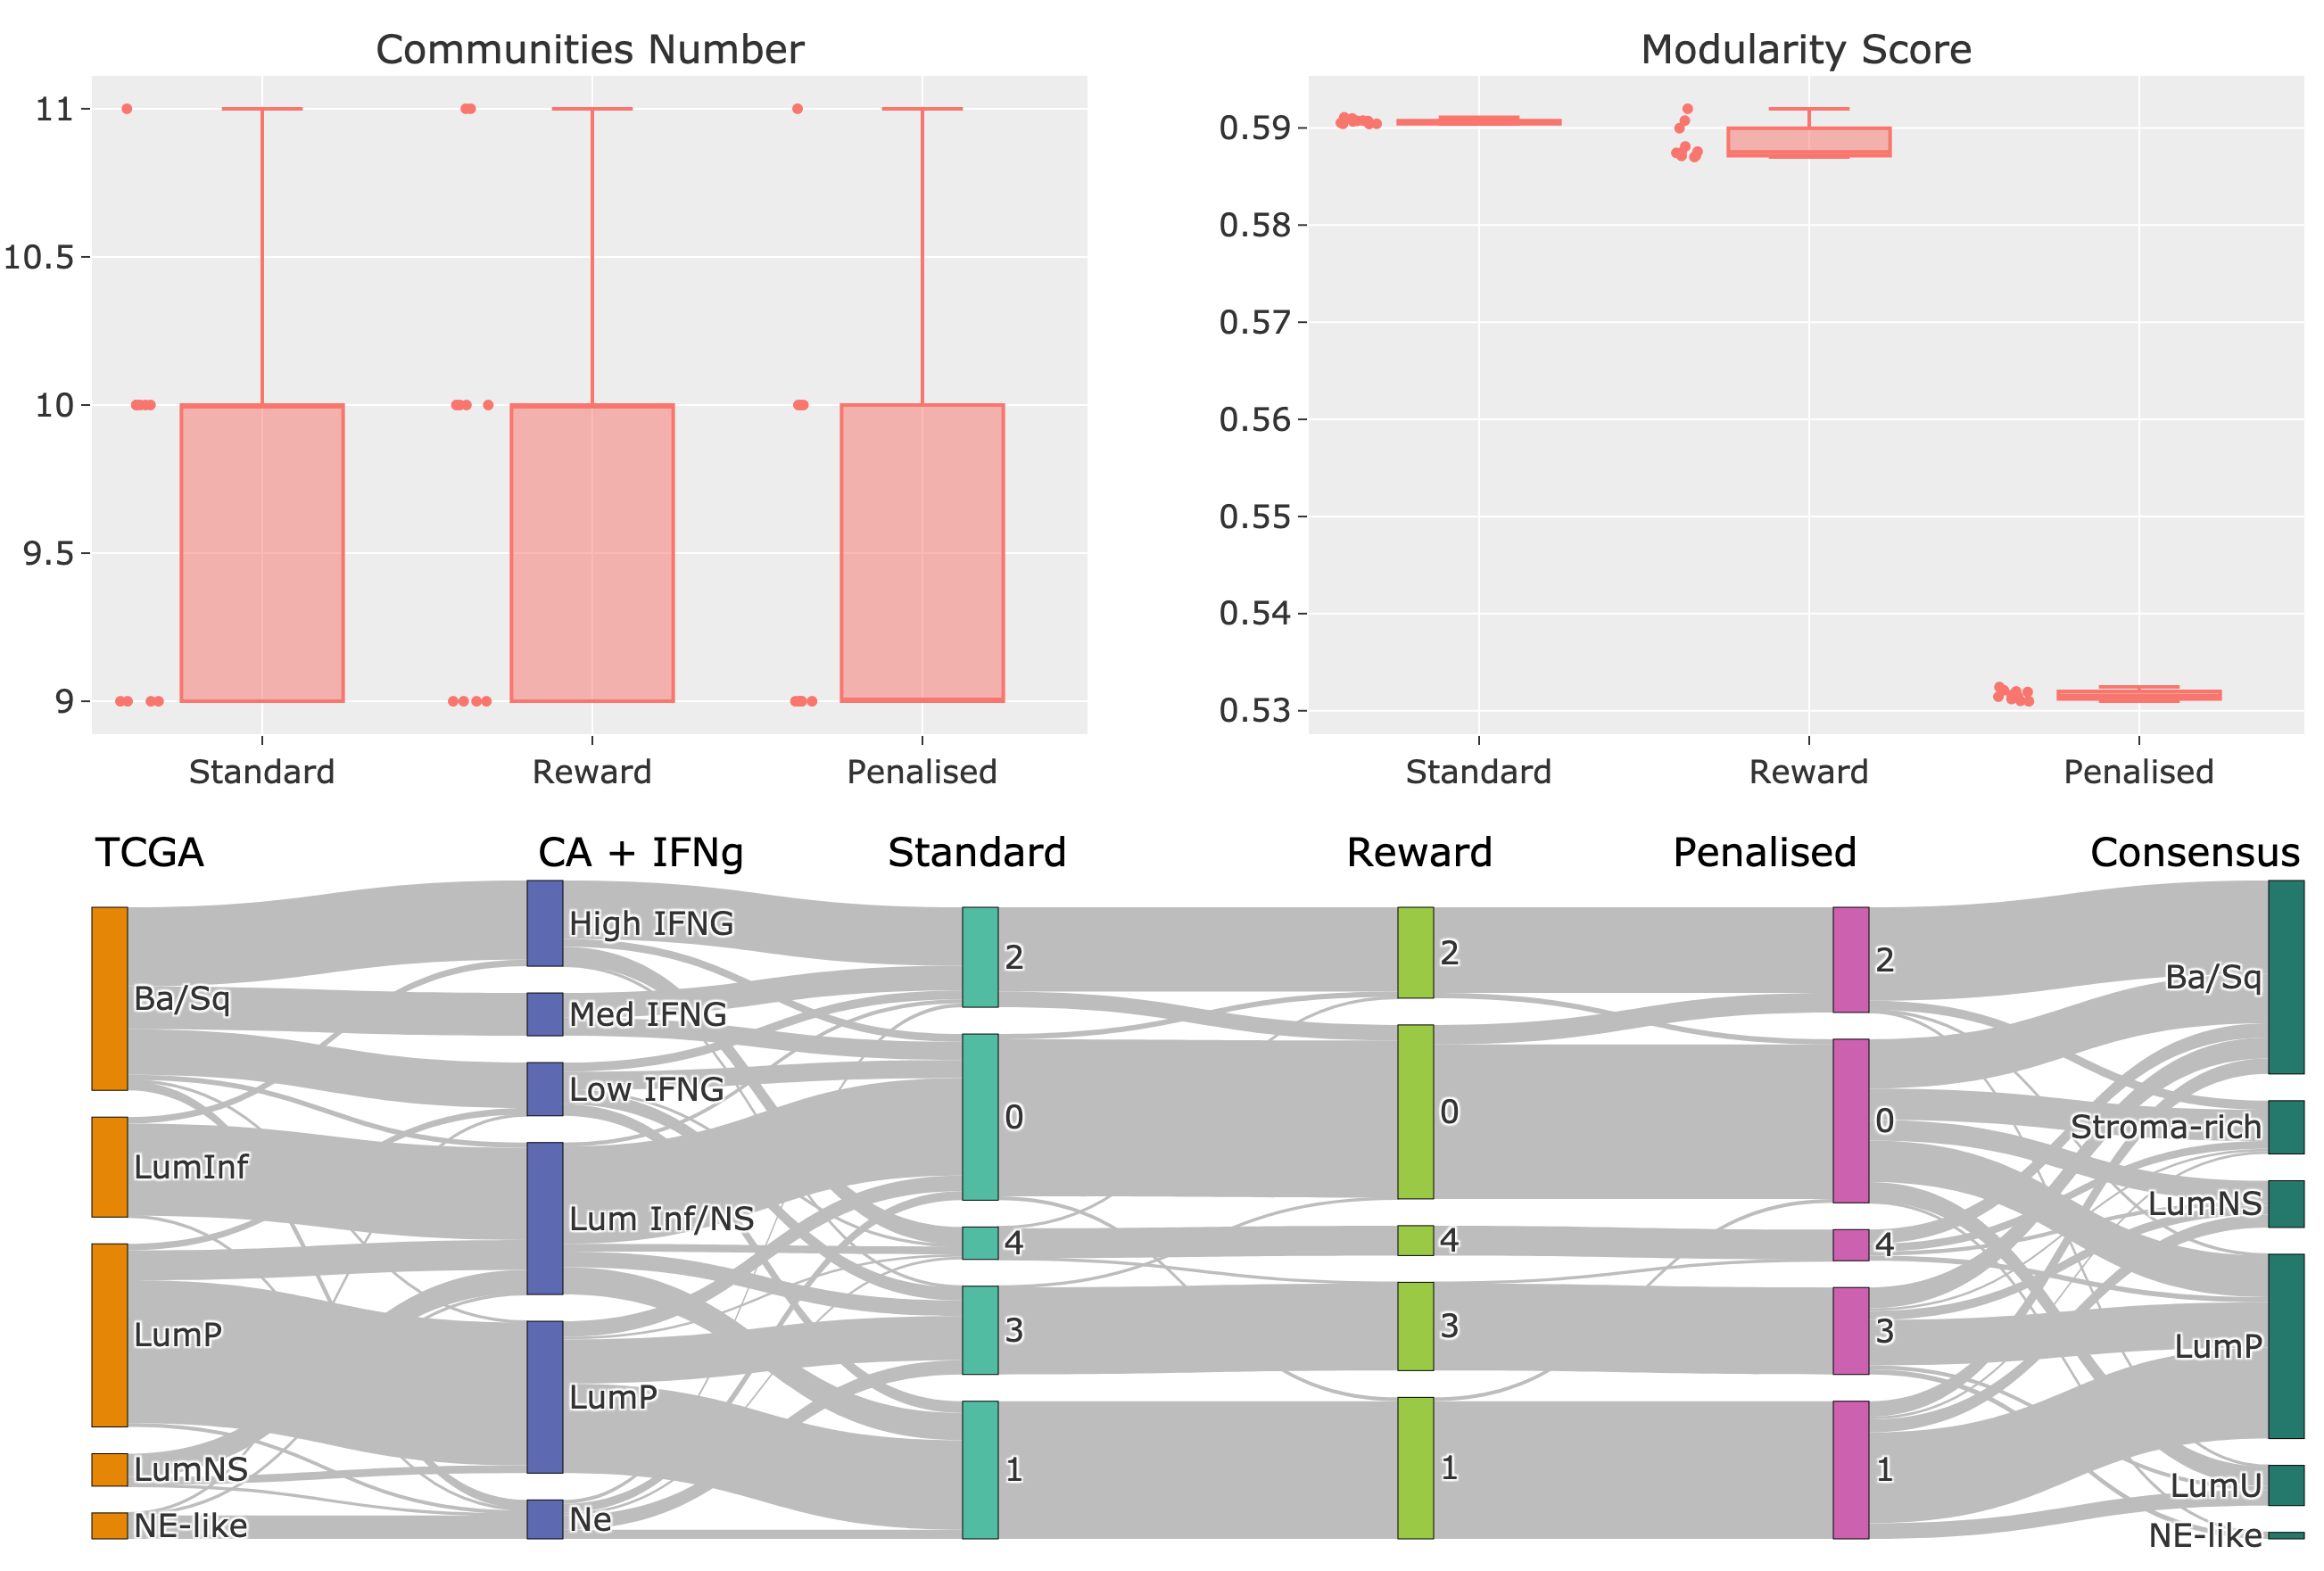
\includegraphics[width=1.0\textwidth,height=0.7\textheight,keepaspectratio]{Sections/Network_I/Resources/P0/Ldn_Sky_TF_50_RawKMeans_K5_v3.png}
    \caption{Overview of the MIBC stratification using P0 dataset.}
    \label{fig:N_I:p0_sky_leiden}
\end{figure}

It is striking the lack of change across the subtypes derived from the three different network as seen in \cref{fig:N_I:p0_sky_leiden}. Cluster \textbf{2} holds most of the High INFG (from CA+INFG), group \textbf{0} is a mixed of the other Basal groups combined with the luminal infiltrated and \textbf{4} is a small subset of High IFNG. The luminal groups are combined in two clusters \textbf{3} and \textbf{1}.


% From the Sankey plot it can be seen that the High IFNG group (CA+IFNg) is contained across the 3 networks in cluster \textbf{2}. Groups \textbf{2} in Standard and Penalised are similar and formed mostly from Ba/Sq groups while cluster \textbf{1} (Reward) has additional samples from LumInf/NS\footnote{Would this mean that by increasing the weight values more samples are added to the group? While pruning edges removes some of the noise?}. The cluster \textbf{0} from the Standard network resembles to the LumInf/NS group from the CA+IFNG classification, being a mixed of samples. Group \textbf{ 0} (Reward and Penalised) and \textbf{1} (Standard) contains samples which previously were considered Luminal samples. Lastly, cluster \textbf{4} contains a consistent number of samples which previously classified as High IFNG.

Overall, the comparison between classifications shows that the network approaches exhibit different subtypes from the other traditional methods. Several samples change group membership in the three different networks, but there are no large changes. As in the previous subsection, this suggests that the weight modifiers strategies have little effect on the subtyping.

% Community analysis
\subsection{Community analysis}

Previous results with tumour networks (Section \ref{s:N_I:tum}) showed that the weight modifiers do have an effect on the network metrics but little effect on the MIBC subtyping. A natural next step is to analyse the changes in communities when a modifier is applied. There are a few questions to answers 1) How do the communities change? 2) Is there a difference in mutation burden? 3) How much the gene expression differs? 

\begin{figure}[H]
    \centering
    \begin{subfigure}[!t]{1.0\textwidth}
        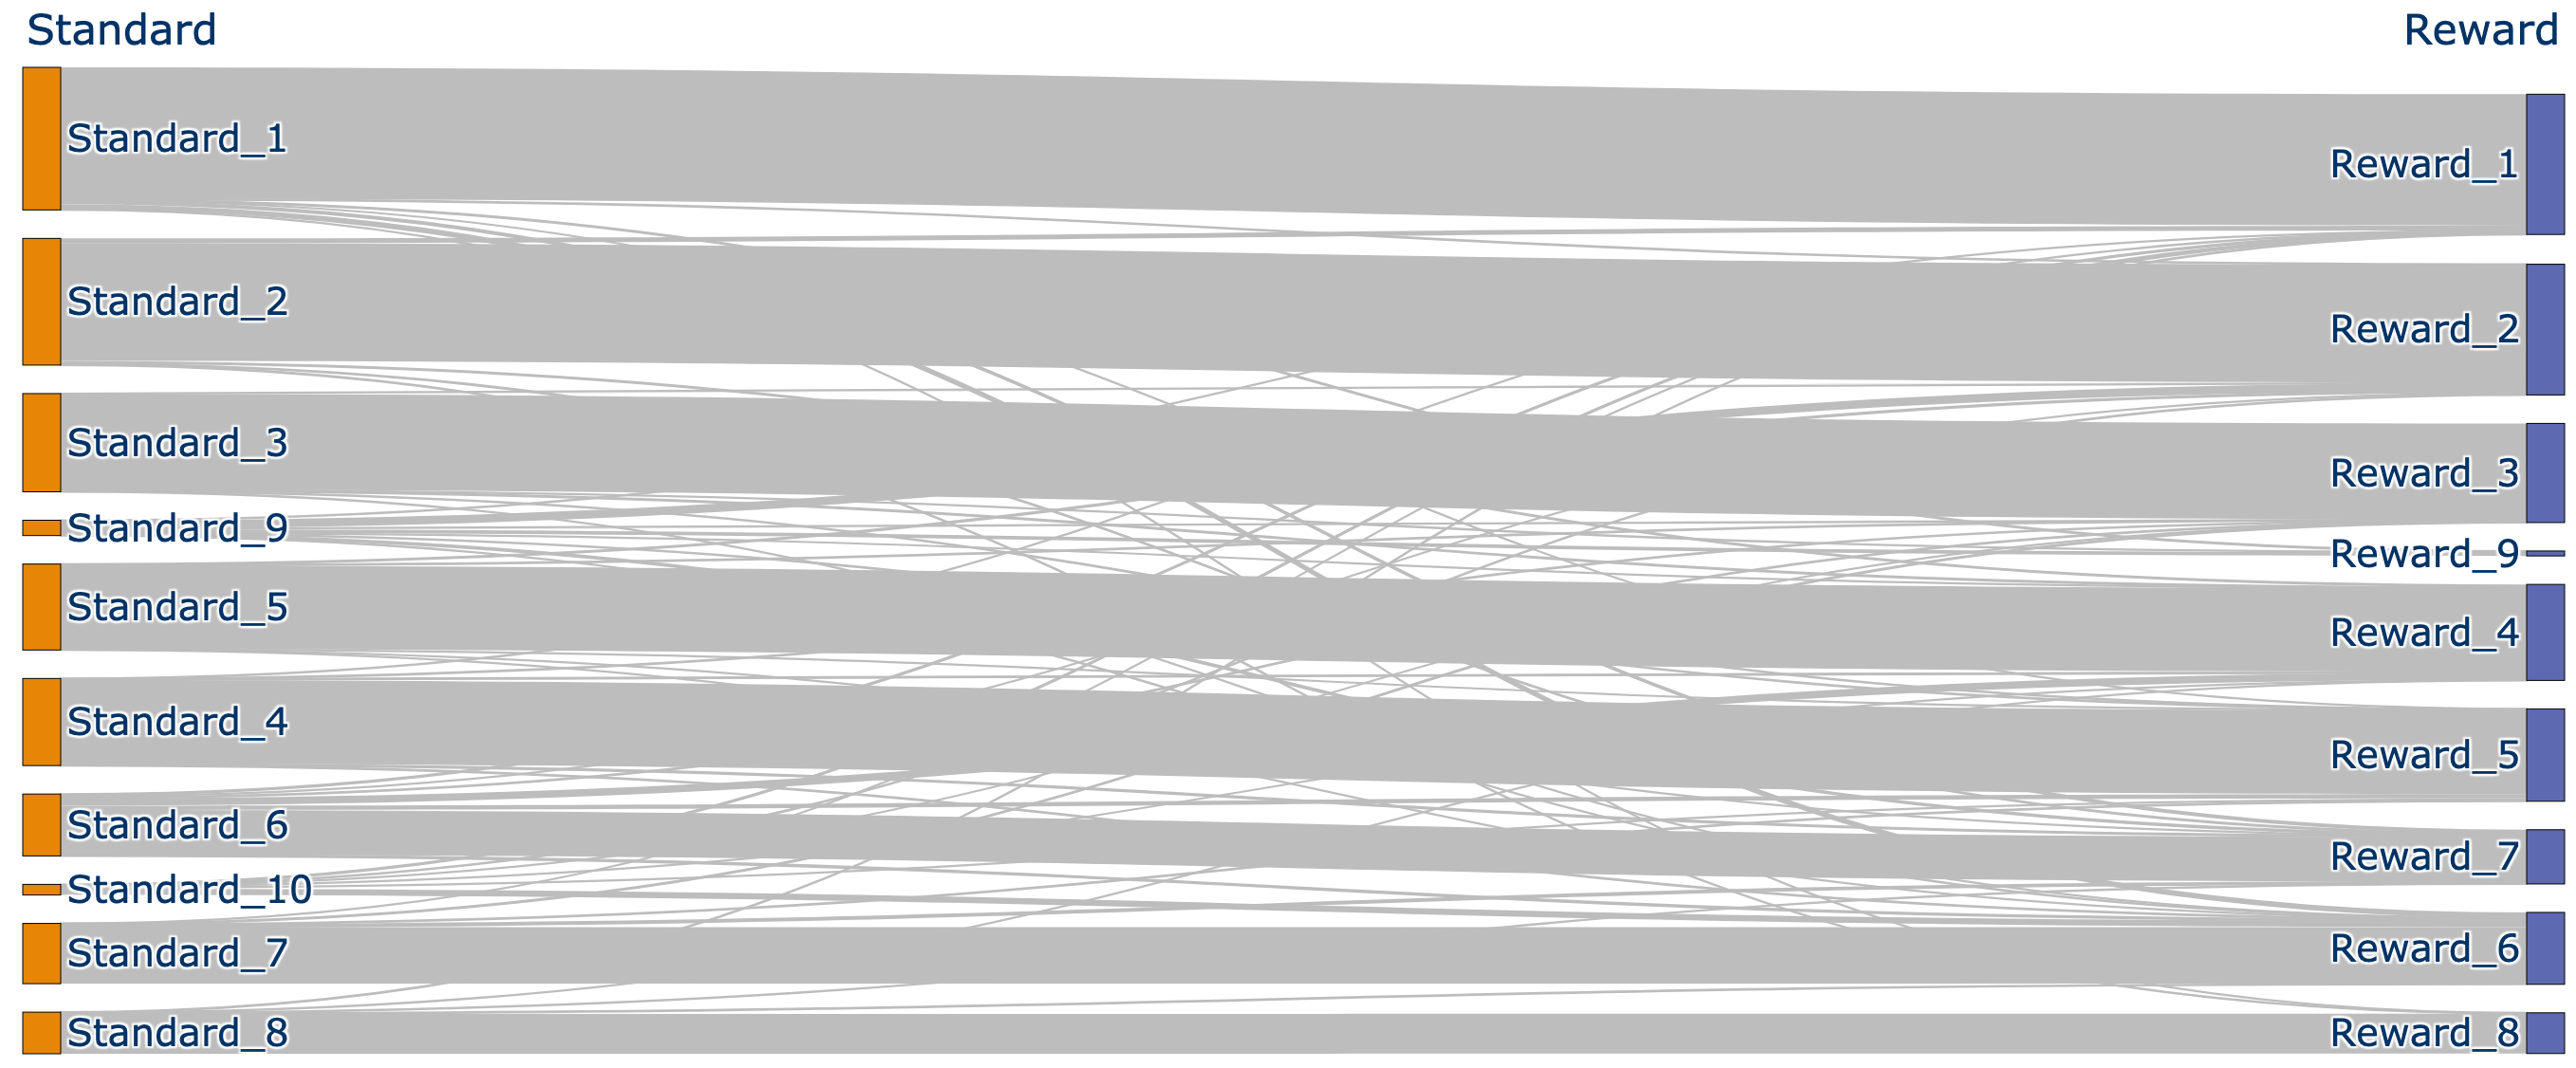
\includegraphics[width=\textwidth,keepaspectratio]{Sections/Network_I/Resources/P0/Comms/Sky_Comm_Comp_4K_v3.png}
        \caption{Gene changes}
        \label{fig:N_I:p0_chg_sankey}
    \end{subfigure}
    \begin{subfigure}[!t]{1.0\textwidth}
        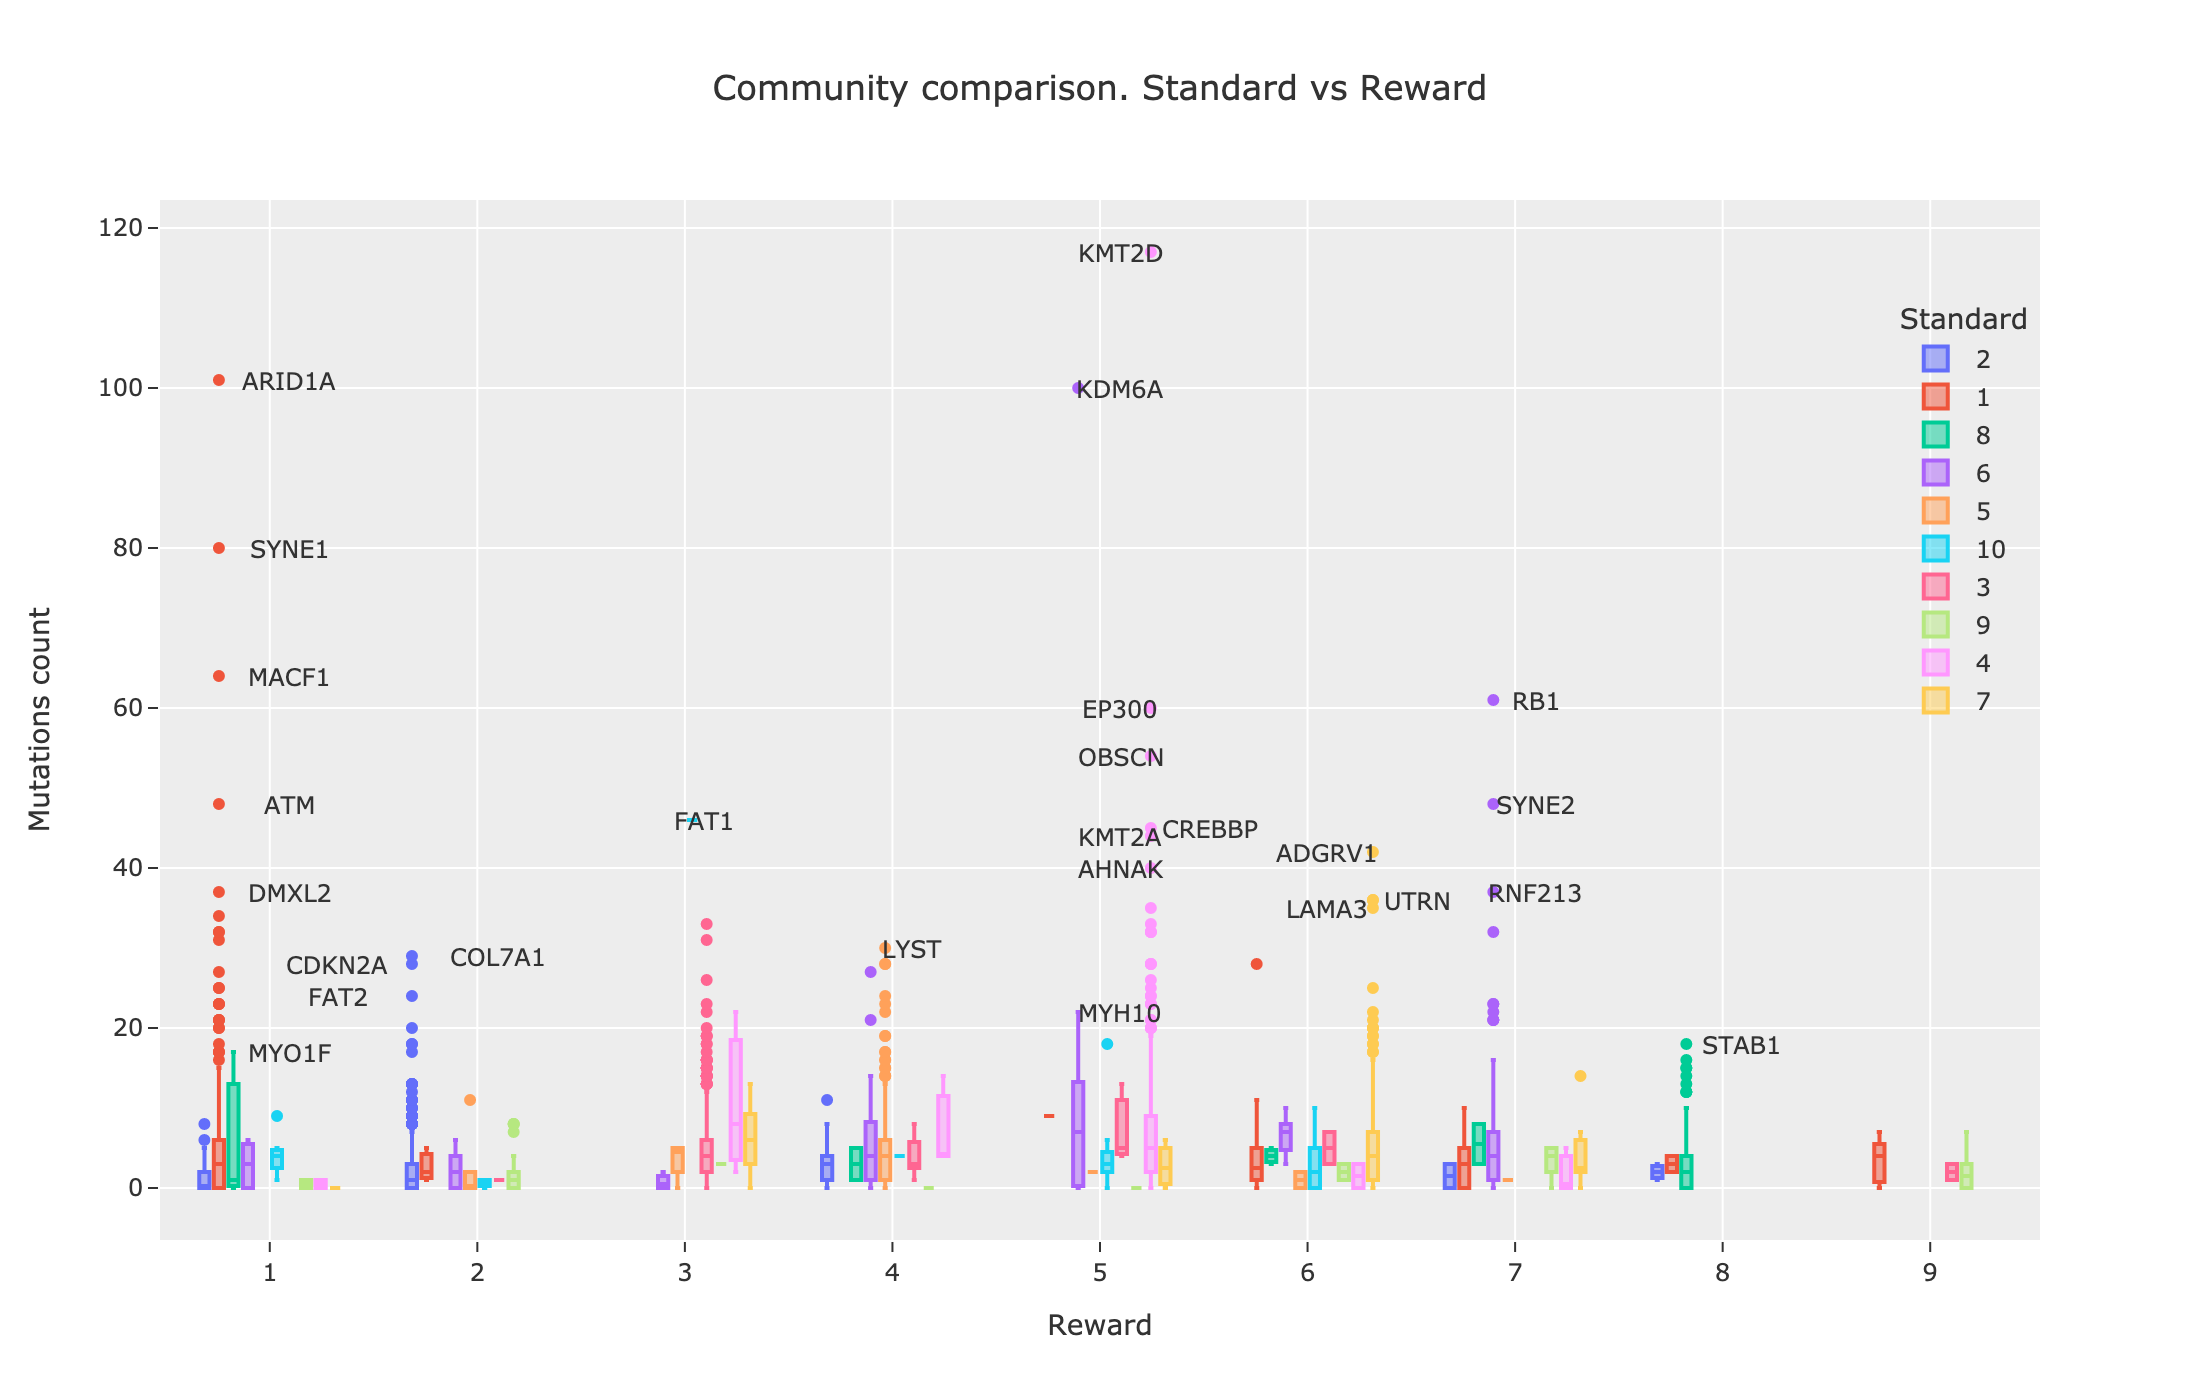
\includegraphics[width=\textwidth,keepaspectratio]{Sections/Network_I/Resources/P0/Comms/Mut_Comm_Comp_4K_v3.png}
        \caption{Mutation representation}
        \label{fig:N_I:p0_chg_mut}
    \end{subfigure}
    \caption{Gene communities changes}
    \label{fig:N_I:p0_comm_chgs_1}
\end{figure}
\begin{figure}[H]
    \centering
    \begin{subfigure}[!t]{1.0\textwidth}
    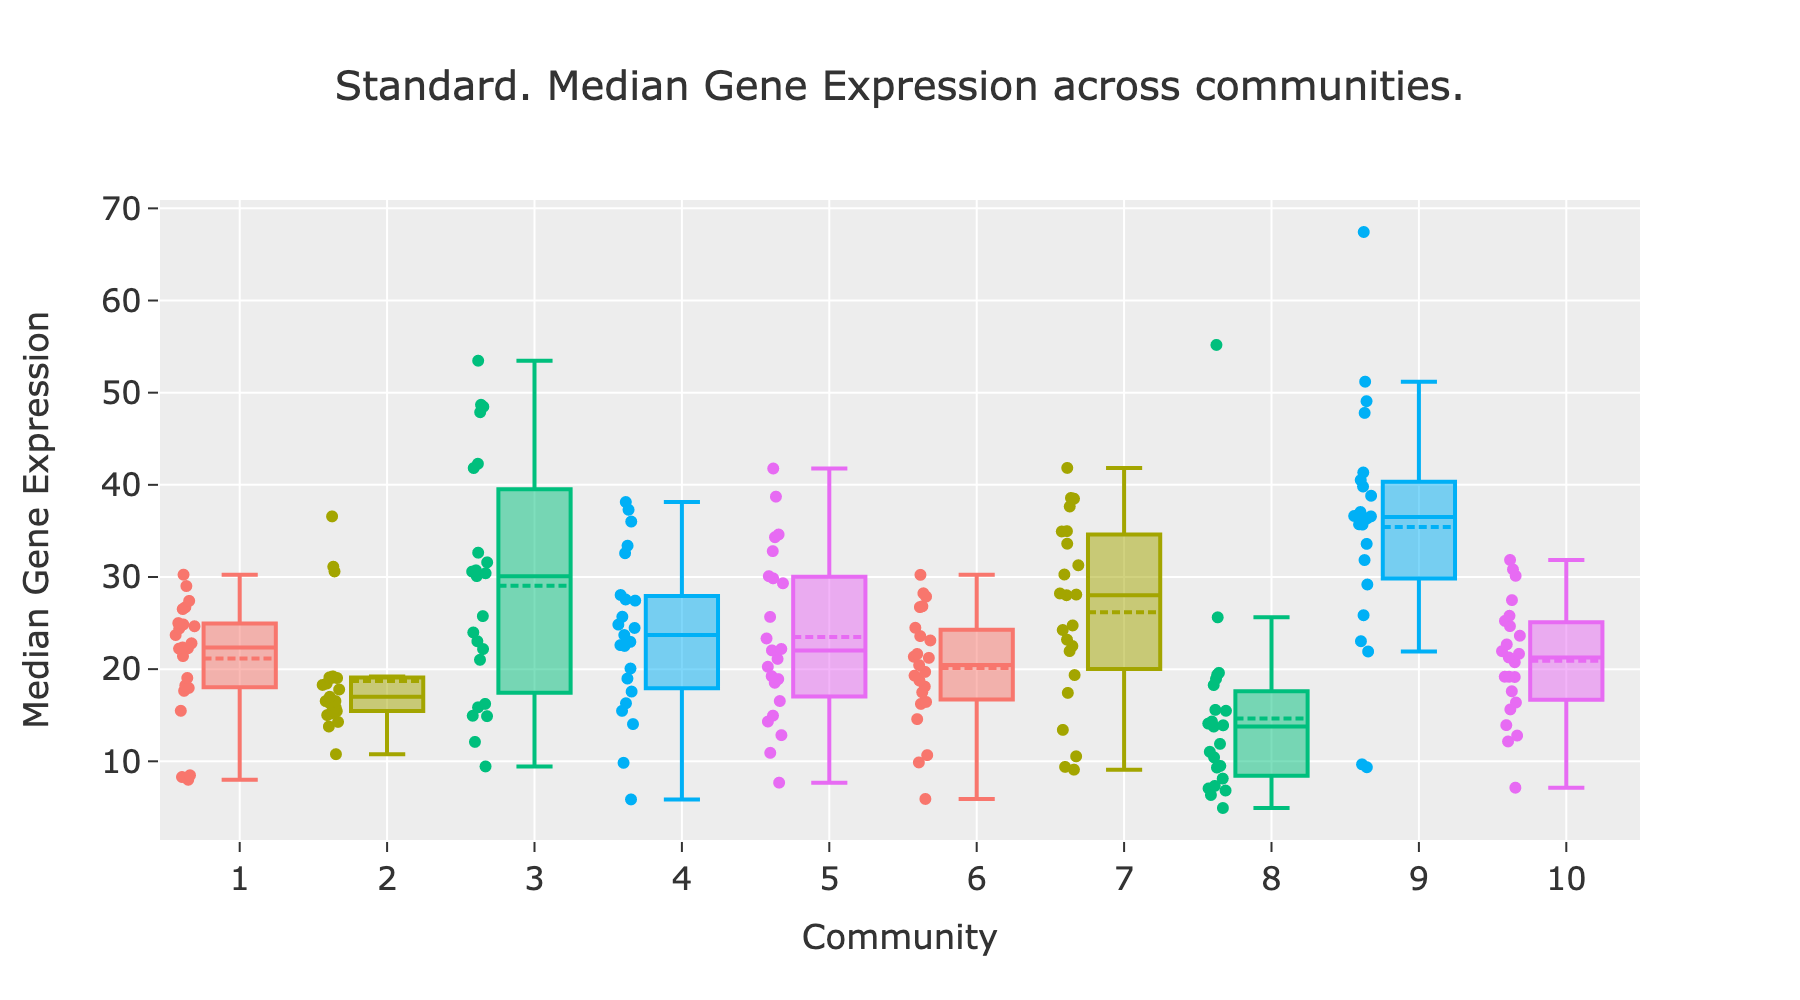
\includegraphics[width=\textwidth,keepaspectratio]{Sections/Network_I/Resources/P0/Comms/P0_standard_4K_50TF_med.png}
        \caption{Standard expression values}
        \label{fig:N_I:p0_chg_std_exp}
    \end{subfigure}
    \begin{subfigure}[!t]{1.0\textwidth}
        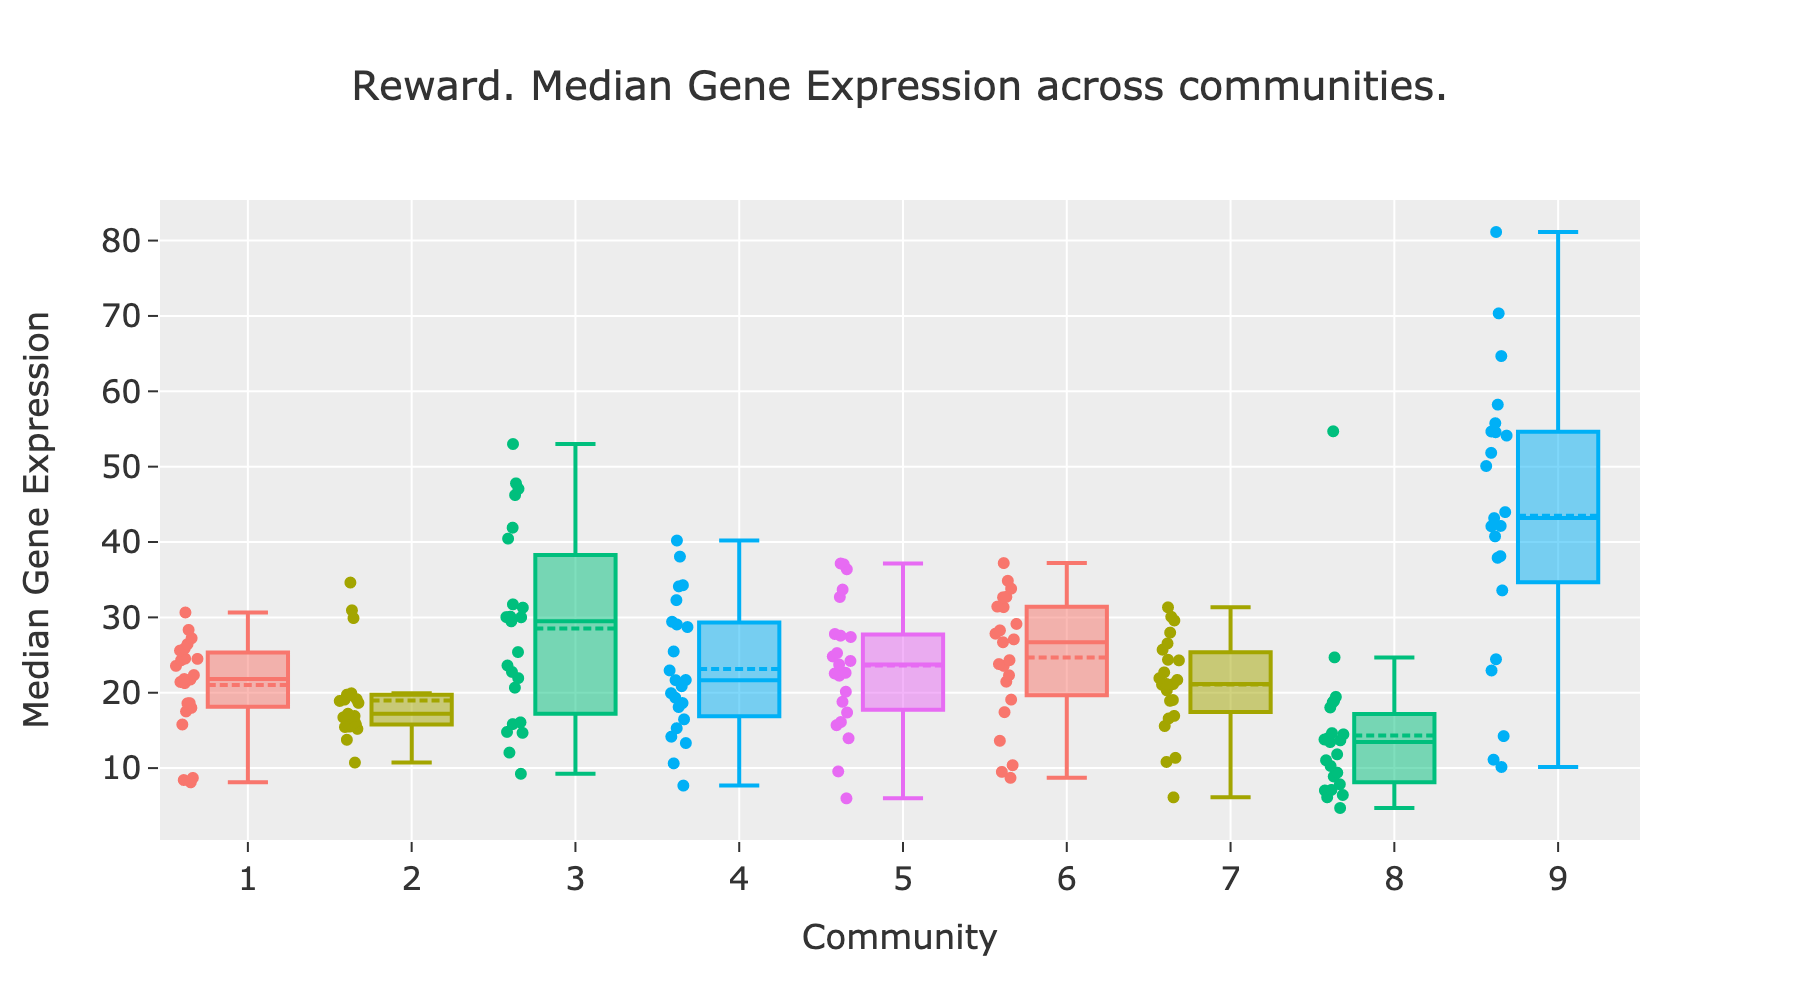
\includegraphics[width=\textwidth,keepaspectratio]{Sections/Network_I/Resources/P0/Comms/P0_norm3_4K_50TF_med.png}
            \caption{Reward expression values}
            \label{fig:N_I:p0_chg_rwd_exp}
    \end{subfigure}
    \caption{Gene communities changes.}
    \label{fig:N_I:p0_comm_chgs_2}
\end{figure}



% How the communities are sincronise
To facilitate analysis, and guided by the Modularity Score, the standard and reward networks have been selected for community comparison; network of 4K genes, with 50 edges for TF and 3 per standard gene. A common challenge in unsupervised learning is the inconsistency in group labelling across different models. Typically, groups are labelled in descending order of their size. However, this approach leads to discrepancies in community labels between the standard and reward networks, complicating the analysis. To address this, community labels are synchronised by using the standard network as a reference for community numbering. Each community in the standard network is then paired with the most similar community in the reward network, based on the highest representation (i.e., the number of genes). This corresponding community in the reward network is then assigned the label from the standard network for consistency.

% Reward modifier is not powerful enough
The sankey in \cref{fig:N_I:p0_chg_sankey} in shows how the genes change communities from the standard to the reward network. The biggest change is represented by the lack of community 10 in the reward network, otherwise the communities remarkable simillar. Figures \cref{fig:N_I:p0_chg_rwd_exp,fig:N_I:p0_chg_std_exp} show the median gene expression across the communities for the two networks. Communities 1 and two are almost unchanged in the reward network while in the others the spread of the median expression is affected. The largest difference is in community 9 and 3.  

Figure \ref{fig:N_I:p0_chg_mut} displays the number of mutated genes (Y) in each reward network's community. For each group it can be usually notice that the there are a large number of mutated genes from the same community. Community 1 has a large number of mutations in the standard network and it receives a few more mutated genes from com 2 (standard). Community 4 has lots of mutated genes in the standard but it receives a few from com 6 as well. Communities 8 and 9 have few mutated genes which can be in part explained by their relative small size. Overall, the reward modifier is the trigger of the community changes but it is not powerful enough to set off large community migrations.


Figure \ref{fig:N_I:p0_chg_mut} is a suitable plot to show that most communities have a higher number of mutated genes between the weight modifiers, but it is not suitable too check if the reward modifier affected the genes with the higher mutation burden. Thus, are the genes with the highest mutation count grouped together? In \cref{fig:N_I:p0_mut_burden} it shows the mutation burden across communities. In the standard, communities 1, 2, 3, 4 and 5 have the highest number of genes mutated and it can be noticed that all have the same trend a sharp decline after mutation burden $>1$; community 4 having the highest number of highly mutated genes. Similar trends can be noticed in the reward network but communities 2,3,4 have a similar slope. In addition, community 9 has just a few mutation with low burden, while 6 and 7 are better separated in the reward. This changes suggests that the highly mutated genes are the ones changing communities.


% Conclusion 1 - Weight modifiers work
Overall, the community analysis shows that the reward modifier works, there are changes between communities and this is given by the mutated genes, especially the ones with a high burden. However, the modifier does not have enough power to cause large changes which may be due to weight modifier shape see \cref{fig:N_I:modifiers}.


\begin{figure}[!htb]
    \centering
    \begin{subfigure}[b]{1.0\textwidth}
        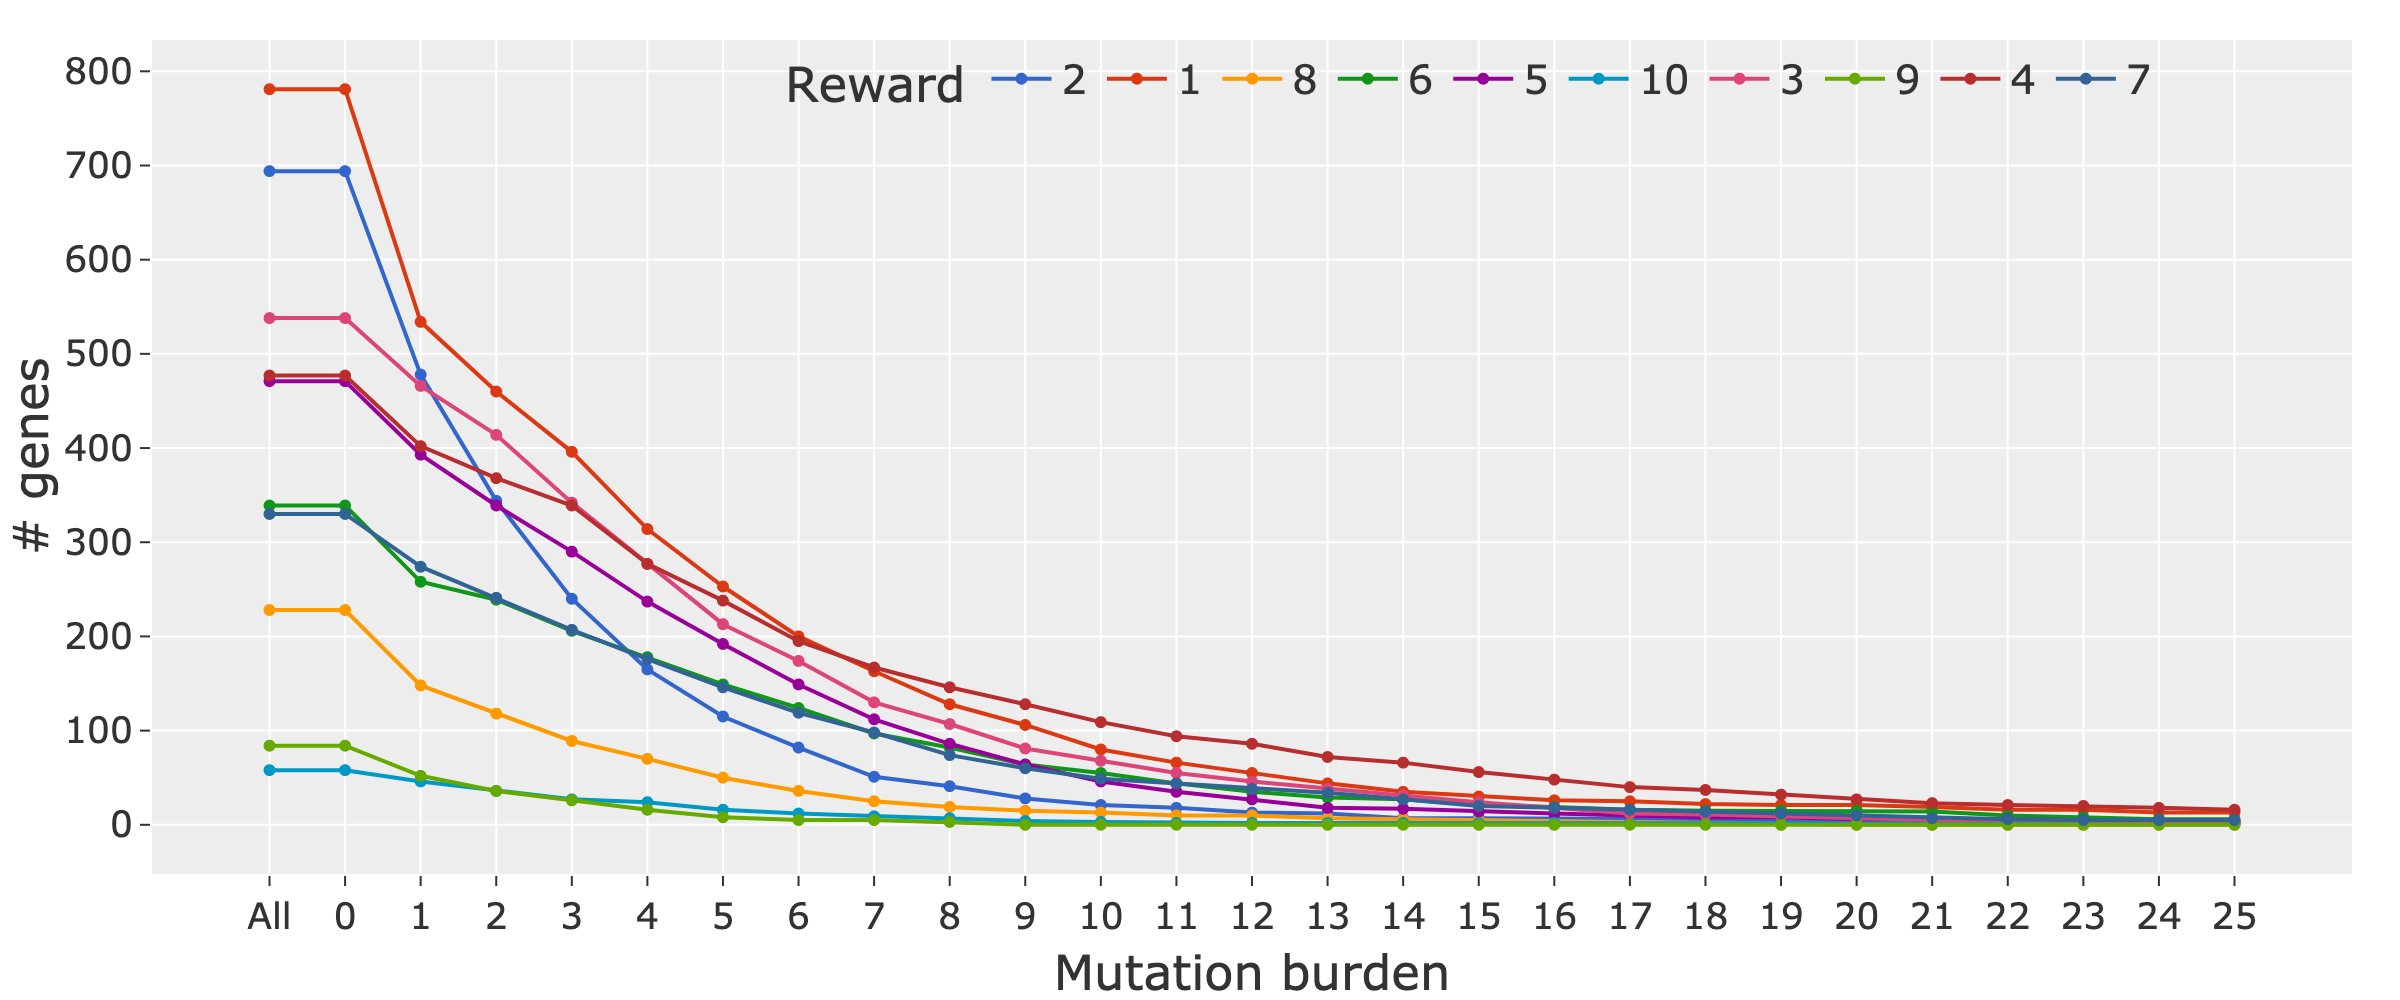
\includegraphics[width=\textwidth,keepaspectratio]{Sections/Network_I/Resources/P0/Comms/Mut_evo_Std_4k_v3.png}
        \label{fig:N_I:p0_std_mut_burden}
        \caption{Standard}
    \end{subfigure}
    \begin{subfigure}[b]{1.0\textwidth}
        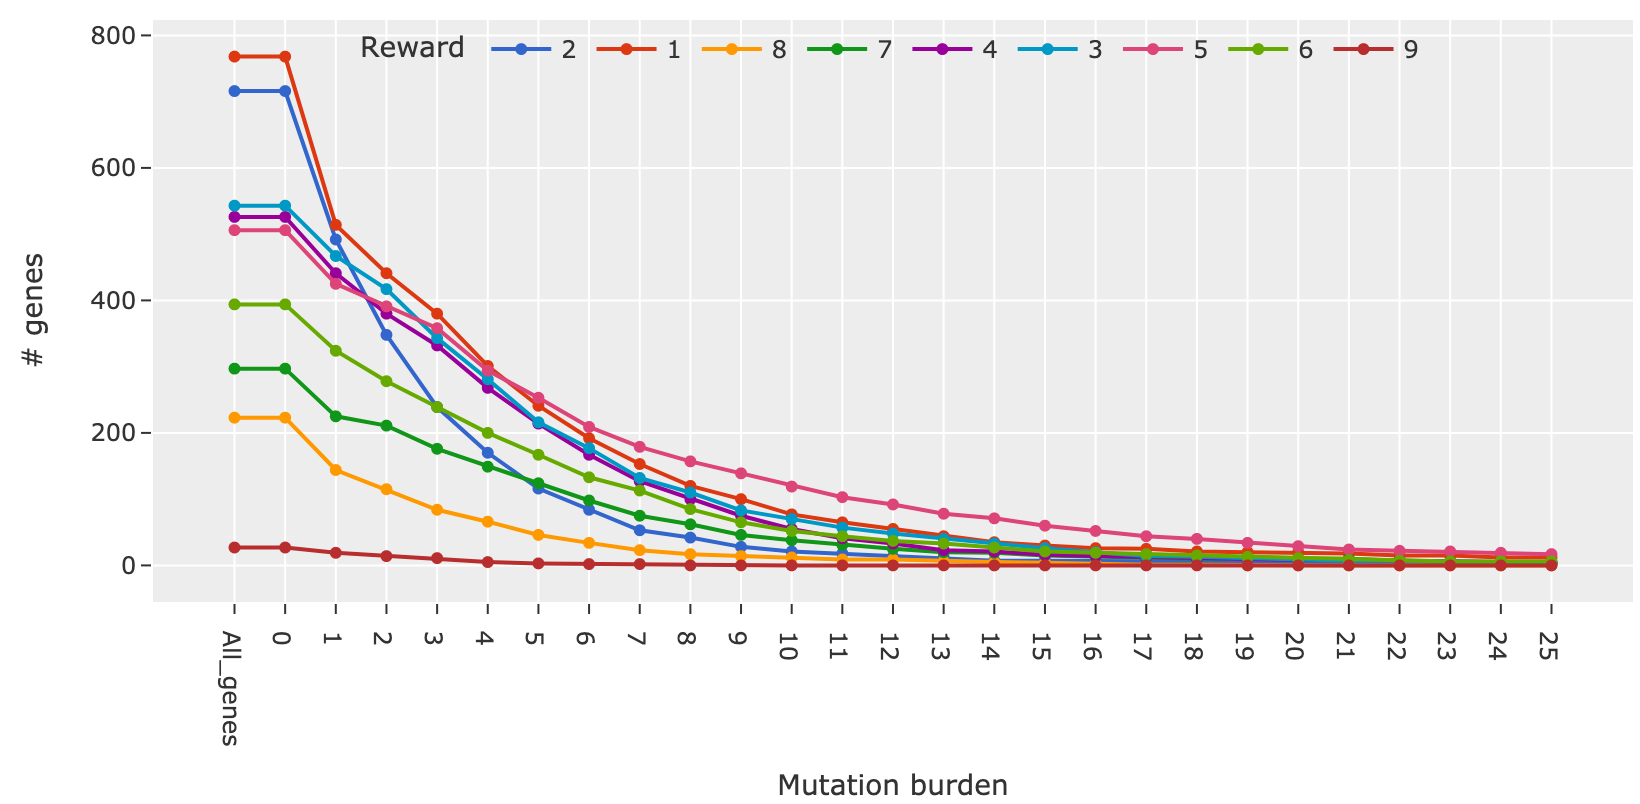
\includegraphics[width=\textwidth,keepaspectratio]{Sections/Network_I/Resources/P0/Comms/Mut_evo_Rwd_4k_v3.png}
        \caption{Reward}
        \label{fig:N_I:p0_rwd_mut_burden}
    \end{subfigure}
    \caption{Mutation burden per communities}
    \label{fig:N_I:p0_mut_burden}
\end{figure}


\subsection{Gene representation}

It is worth remembering that the network is built on the P0 data and then the genes extracted from with ModCon are used to stratify the tumour dataset. The two types of data is expected to have differences in gene expression, some of the genes may be expressed in the P0 data but not in the tumour and vice-versa. Therefore, it is important to understand how well the genes selected are represented through the network approach (ModCon and MEV) in the tumour dataset. 


% Conclusion 2 - Poor representation
\Cref{fig:N_I:p0_mev_rep} shows that representation for each community. In \cref{fig:N_I:p0_mev_sel_rep} shows the genes selected are represented in the most varied genes (in TCGA) while \cref{fig:N_I:p0_mev_all_rep} in all $\sim13K$ most expressed genes. From the two sub-figures it can be clearly seen that using just the most varied genes was missing a large number of genes. Nevertheless, there are is still a few genes missing when all the expressed genes are used. One possible explanation is that a larger dataset is needed to form the network which includes a molecular representation of the basal groups; i.e. undifferentiated samples from non-tumours. Another reason for this is that the gene filtering using in \cref{s:cs:pre-processing} is too aggressive, too many genes are discarded which will lead of a poor mismatch between tumour and non-tumour expressed genes. The difference in gene filtering is discussed in section \cref{s:N_II} (section in the last chapter).

\begin{figure}[!htb]
    \centering
    \begin{subfigure}[b]{0.47\textwidth}
        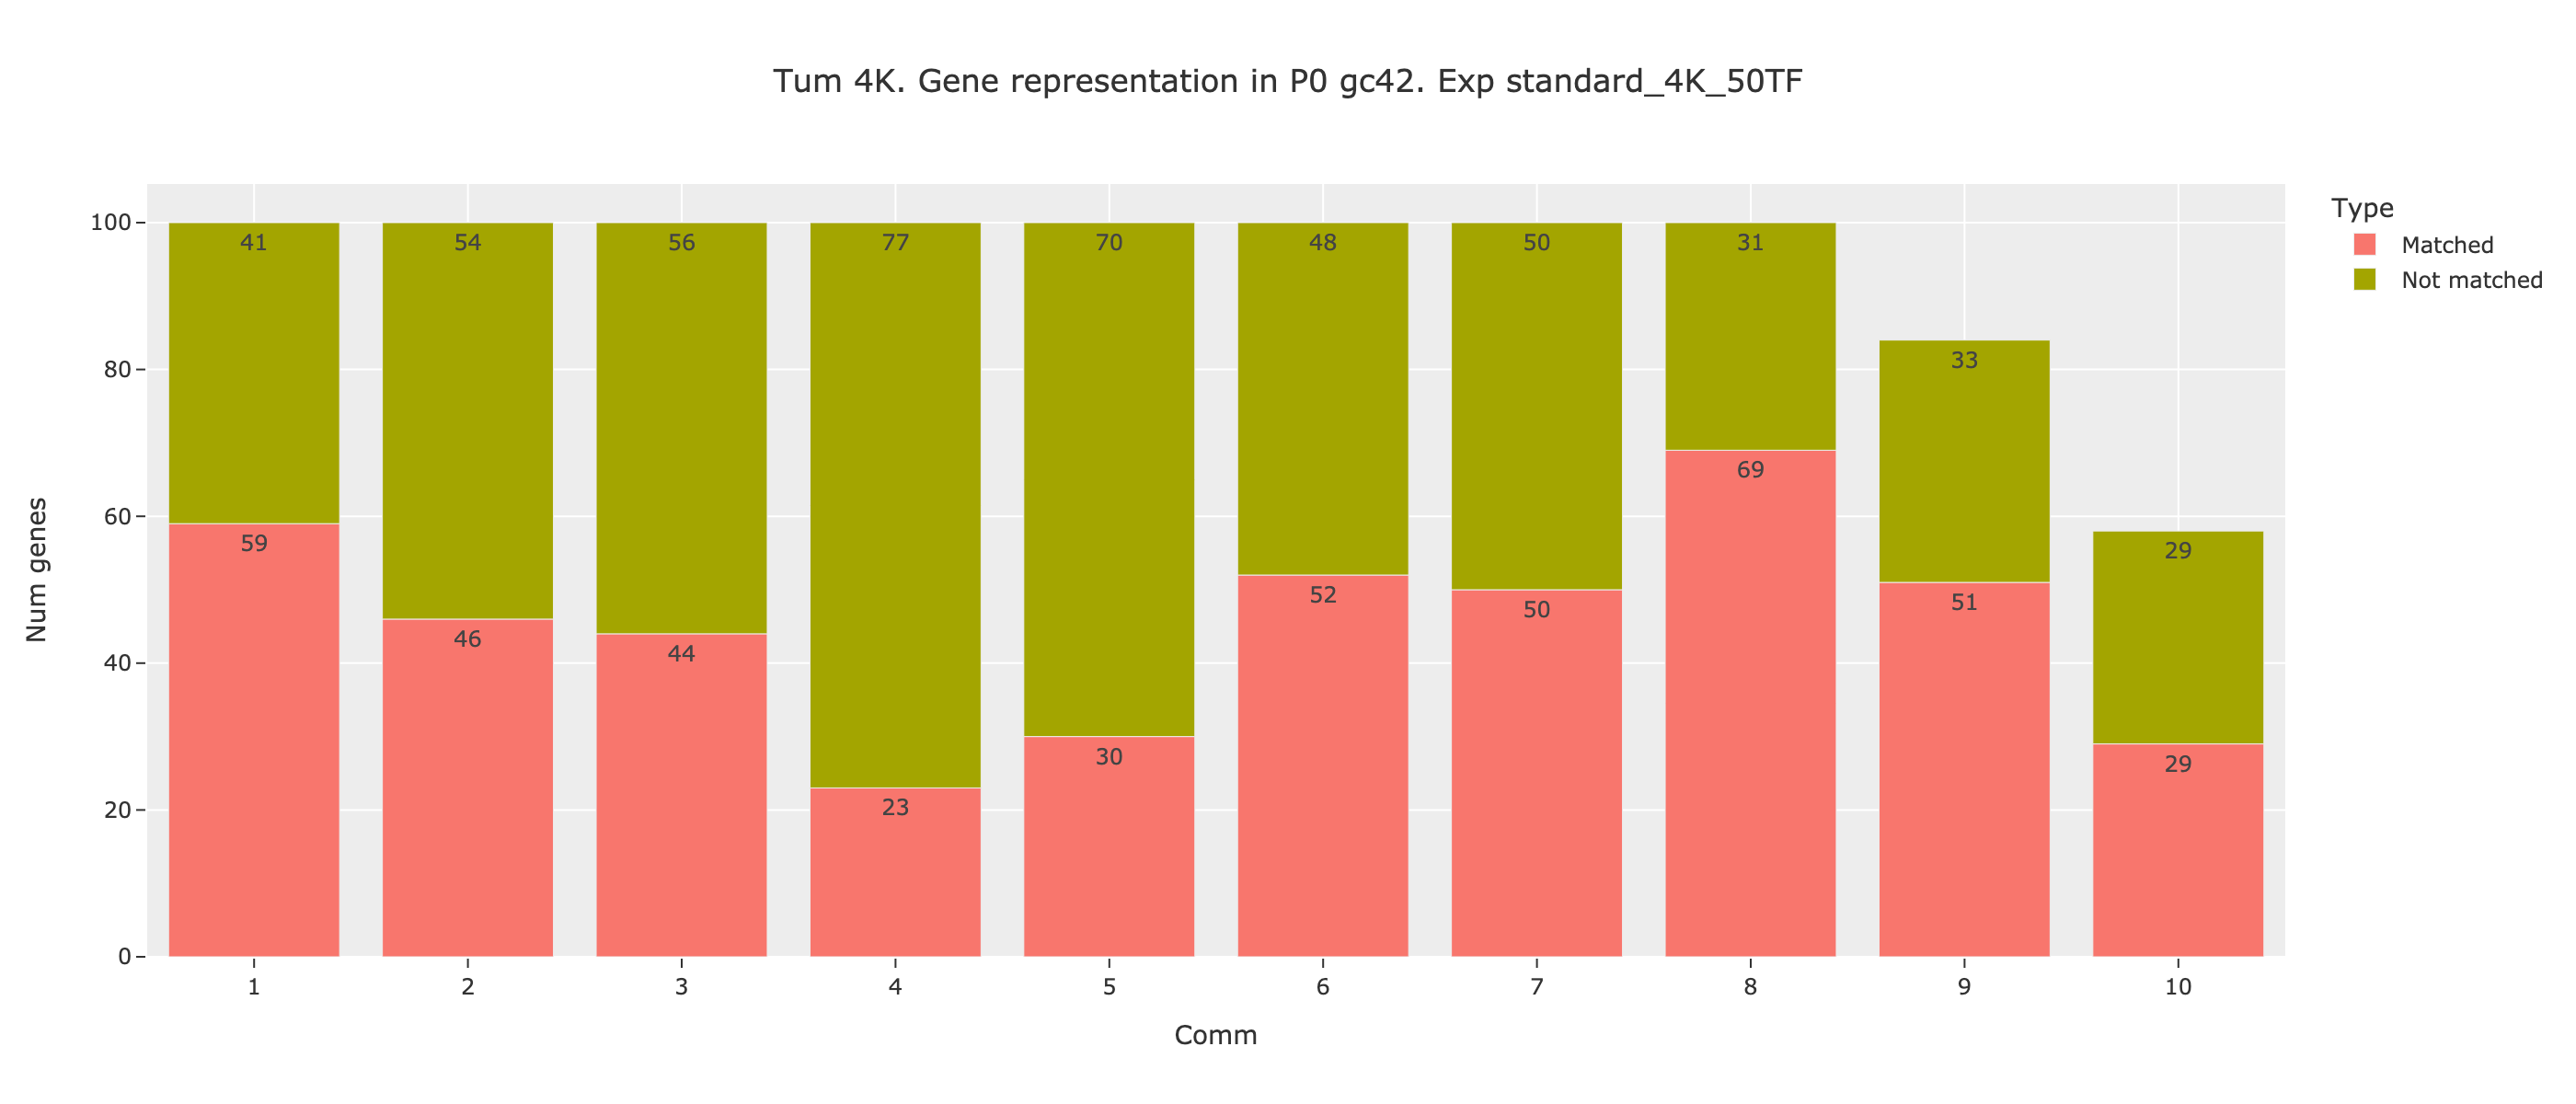
\includegraphics[width=\textwidth,keepaspectratio]{Sections/Network_I/Resources/P0/4K_p0_modConMev_rep_standard_4K_50TF_v3.png}
        \caption{The most relative varied genes}
        \label{fig:N_I:p0_mev_sel_rep}
    \end{subfigure}
    \begin{subfigure}[b]{0.47\textwidth}
        \centering
        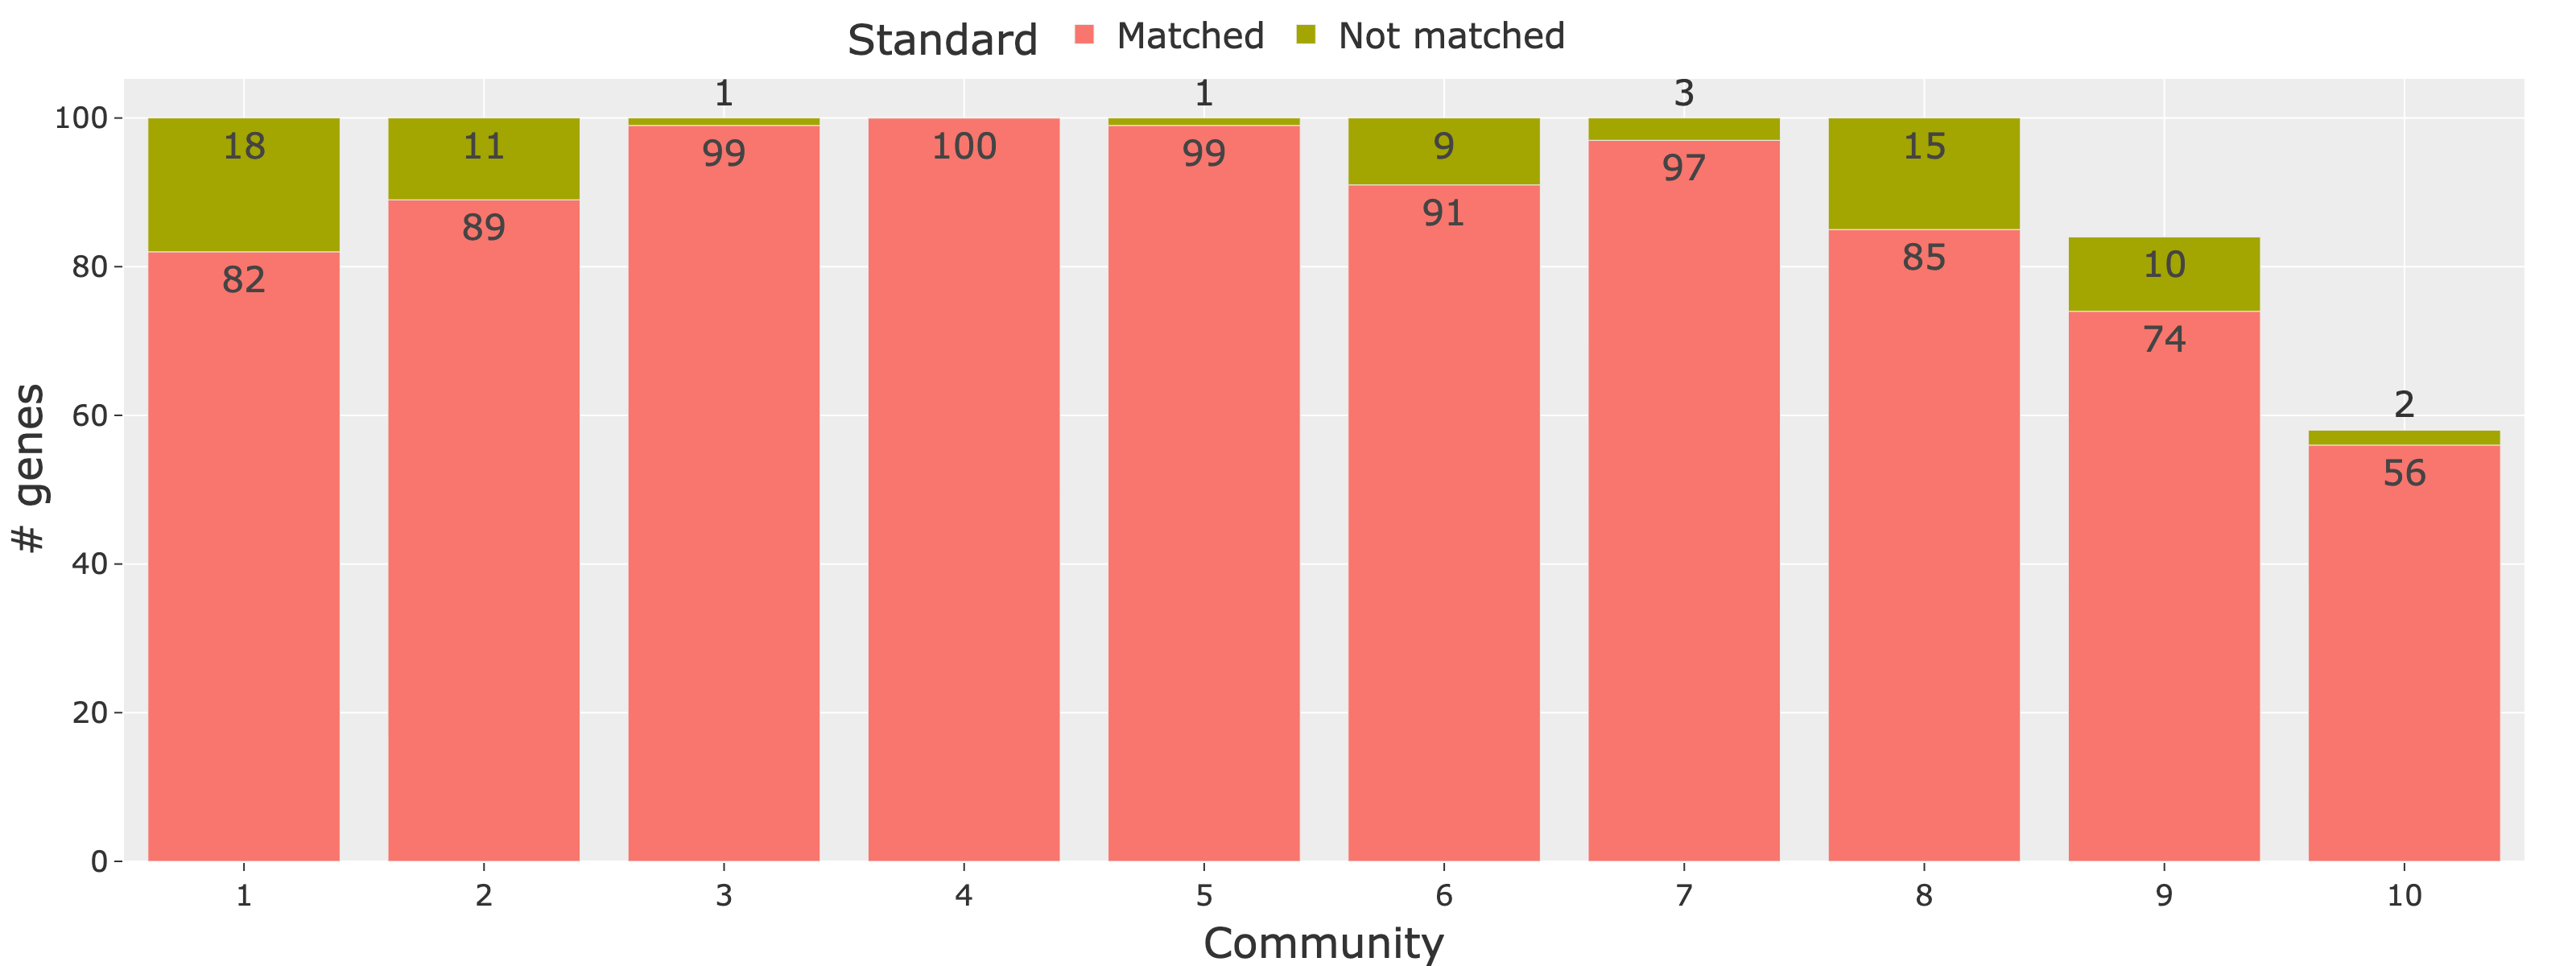
\includegraphics[width=\textwidth,keepaspectratio]{Sections/Network_I/Resources/P0/13K_p0_modConMev_rep_standard_4K_50TF_v3.png}
        \caption{All the genes expressed}
        \label{fig:N_I:p0_mev_all_rep}
    \end{subfigure}
    \caption{Genes found in the tumour dataset for each network community. The top 100 genes are selected by ModCon score. A) Is when the tumour dataset is restricted to the top most varied genes B) Includes all the expressed genes in the tumour dataset. }
    \label{fig:N_I:p0_mev_rep}
\end{figure}


\subsection{Summary}

This section contains the first attempt in the project to integrate the non-healthy molecular information into MIBC subtyping by building a network on the P0 sample and using the derived communities for MIBC stratification. The networks generated utilised the standard, reward, and penalised modifiers, with a minimum degree of 3 for standard genes and 50 for TFs. There are several limitations with the method presented in this section. The dataset consists only of P0 samples (only 23), so the network does not represent the undifferentiated tissue. In addition, the gene expression for both tumour and non-tumour datasets was aggressively filtered by keeping only the genes expressed in 90\% of the samples. This led to a poor representation in the TCGA dataset of the genes selected through the networks.

The minimum degree of 50 for TFs was pseudo-randomly chosen with the hope of prioritising the TFs in the network. This was based on the assumption that the Leiden community detection algorithm is agnostic to the number of connections per node. Given the poor results in the MIBC subtyping, this assumption came under scrutiny. The next section studies the effects on the network pipeline, and implicitly on Leiden, when a subset of genes is prioritised at the edge pruning stage. In addition, the MEV only uses the gene expression for tumours, without fully integrating the two gene expression datasets. While this section did not generate useful biological findings, it was crucial in the development process.



% % Reason 2 - Scatter biological pathways 
% Further on, when we look at the biology of each community we could see that there a lot shared pathways across communities. This include PDGF, CCKR, apoptosis and others. This gives the impression that the approach developed did the contrary from the intended behaviour, instead of isolating the biological processes it scattered through the network. The pathways were discovered through the Gene Ontology tool using PANTHER Pathway option and \textbf{no correction}; the latter because the majority of the genes inputted were \textbf{not} given significant results. This further strengthen our intuition that this approach is not providing the intended results.

% Figures I need to support for the above argument:
% \begin{itemize}
%     \item Pick 2-3 pathways from the ones found and highlight in the network.
%     \item Maybe put the Network with annotations?
% \end{itemize}

% % Reason 3 - Effect of the TF. but this really is 
% While performing the biological interpretation, looking at the genes selected by ModCon score, it can be clearly noticed that the TF genes play a major role in the networks. The reason for this is that in this set of experiment we enable 50 edges for each Transcription Factor, thus biasing the network for these genes. Definitely, this parameter have a large impact of ModCon. Therfore, we performed an experiment with a lower number of edges per TF and we found out that there are more communities with fewer communties.
% Figure supporting the above:
% \begin{itemize}
%     \item How many of the genes selected from the ModCon are a TF? Give some stats
%     \item The sub-graph where only the ModCon genes are selected for each community; with the size of the TF \ref{fig:N_1:tf_comp}
% \end{itemize}

